\part{Design, Evaluation, and Optimization}

\chapter{User Stories}
\ChapterLabel{UserStories}
\index{user story}
\index{acceptance criterion}
% \section{How to Use This Chapter}
% Capture stakeholder goals in accessible language. Stories express value and
% acceptance intent; precise obligations belong in Requirements. Give each story
% a stable ID, a priority, and links to one or more requirements that implement it.

\section{User Story Register}
\begin{tabularx}{\linewidth}{L{1.9cm}YL{1.8cm}L{3.4cm}}
\caption{User Story Register\label{Table:UserStories}}\\
\toprule
\textbf{ID} & \textbf{Story and Acceptance Criteria} & \textbf{Priority} & \textbf{Requirement(s)}\\
\midrule
\endfirsthead
\multicolumn{4}{l}{\small\itshape User Story Register (continued)}\\
\toprule
\textbf{ID} & \textbf{Story and Acceptance Criteria} & \textbf{Priority} & \textbf{Requirement(s)}\\
\midrule
\endhead
\midrule
\multicolumn{4}{r}{\small\itshape Continued on next page}\\
\endfoot
\bottomrule
\endlastfoot

\UserStoryID{US-001} &
As a researcher, I want to access the research artifacts so that I can review, reuse, and independently inspect the work. Acceptance: the system provides access to the research paper, available simulation code, and research data while clearly distinguishing raw and processed data artifacts. &
\gls{must} &
\RequirementRef{REQ-B-001}, \RequirementRef{REQ-D-005}, \RequirementRef{REQ-C-001}\\

\UserStoryID{US-002} &
As a researcher or student, I want to explore explanations of the fundamental concepts used in the research so that I can understand the scientific context of the project. Acceptance: the system presents relevant research concepts and provides the physical definitions and units needed to interpret the scientific variables used by the project. &
\gls{must} &
\RequirementRef{REQ-B-003}, \RequirementRef{REQ-D-008}, \RequirementRef{REQ-C-001}\\

\UserStoryID{US-003} &
As a researcher, I want to examine key research figures and trace them back to their supporting data so that I can understand how the reported results were produced. Acceptance: a key figure can be associated with the processing or analysis procedure, relevant scientific quantities and units, source data, and simulation parameters used to produce it. &
\gls{must} &
\RequirementRef{REQ-B-004}, \RequirementRef{REQ-D-006}, \RequirementRef{REQ-D-007}, \RequirementRef{REQ-D-008},    \RequirementRef{REQ-I-001}, \RequirementRef{REQ-C-001}\\

\UserStoryID{US-004} &
As a researcher, I want sufficient data, metadata, and procedural information to reproduce a documented result so that I can independently verify the research. Acceptance: the system provides the required simulation inputs, computational environment and software metadata, raw and processed data relationships, analysis procedures, provenance information, and other documented information needed to reproduce a simulation and its associated analysis. &
\gls{must} &
\RequirementRef{REQ-B-005},    \RequirementRef{REQ-D-004}, \RequirementRef{REQ-D-005}, \RequirementRef{REQ-D-007}, \RequirementRef{REQ-D-008} \\

\UserStoryID{US-005} &
As a researcher, I want to find multiple projects relevant to a topic. Acceptance: the system searches through all projects and returns a list of projects relevant to the query &
\gls{must} &
\RequirementRef{REQ-B-005},    \RequirementRef{REQ-D-004}, \RequirementRef{REQ-D-005}, \RequirementRef{REQ-D-006} \\
%\RequirementRef{REQ-D-010}, \RequirementRef{REQ-D-011}\\

\UserStoryID{US-006} &
As a general member of the population, I want to understand the results of a paper. Acceptance: Scientific terms are defined in plain language. &
\gls{must} &
\RequirementRef{REQ-B-005},    \RequirementRef{REQ-D-004}, \RequirementRef{REQ-D-005}, \RequirementRef{REQ-D-006} \\
%\RequirementRef{REQ-D-010}, \RequirementRef{REQ-D-011}\\

\UserStoryID{US-007} &
As a general member of the population, I want to understand the figures in a paper. Acceptance: Figures and how they relate to the research are described in plain language.&
\gls{must} &
\RequirementRef{REQ-B-005},    \RequirementRef{REQ-D-004}, \RequirementRef{REQ-D-005}, \RequirementRef{REQ-D-006} \\ %\RequirementRef{REQ-D-010}, \RequirementRef{REQ-D-011}\\

\UserStoryID{US-008} &
As a researcher with no web development background, I want to use the system to support my research. Acceptance: Research pages can be made without installation of any tools or writing of any code. &
\gls{must} &
\RequirementRef{REQ-B-005},    \RequirementRef{REQ-D-004}, \RequirementRef{REQ-D-005}, \RequirementRef{REQ-D-006},    \RequirementRef{REQ-I-002}, \RequirementRef{REQ-C-002}\\
%\RequirementRef{REQ-D-010}, \RequirementRef{REQ-D-011}, 

\UserStoryID{US-009} &
As a researcher, I would like to use videos to help convey complex processes in my research. Acceptance: Videos can be uploaded and displayed on the system.&
\gls{should} &
\RequirementRef{REQ-B-005},    \RequirementRef{REQ-D-004}, \RequirementRef{REQ-D-005}, \RequirementRef{REQ-D-006} \\ 
%\RequirementRef{REQ-D-010}, \RequirementRef{REQ-D-011}, \RequirementRef{REQ-I-003}\\

\UserStoryID{US-010} &
As a researcher, I want to easily tell if a paper is relevant to me to decide if I should read more. Acceptance: Researchers can determine the relevance of a paper without reading the paper. &
\gls{should} &
\RequirementRef{REQ-B-005},    \RequirementRef{REQ-D-004}, \RequirementRef{REQ-D-005}, \RequirementRef{REQ-D-006} \\ %\RequirementRef{REQ-D-010}, \RequirementRef{REQ-D-011}\\

\UserStoryID{US-011} &
As a researcher, I want to be able to edit materials related to a paper. Acceptance: Users can edit materials after they have be posted. &
\gls{must} &
\RequirementRef{REQ-B-005},    \RequirementRef{REQ-D-004}, \RequirementRef{REQ-D-005}, \RequirementRef{REQ-D-006} \\ %\RequirementRef{REQ-D-010}, \RequirementRef{REQ-D-011}\\

\UserStoryID{US-012} &
As a third-party researcher, I want to comment on others' research to build scientific discourse. Acceptance: Users can leave public comments on specific materials of a research project. &
\gls{should} &
\RequirementRef{REQ-B-005},    \RequirementRef{REQ-D-004}, \RequirementRef{REQ-D-005}, \RequirementRef{REQ-D-006} \\ %\RequirementRef{REQ-D-010}, \RequirementRef{REQ-D-011}\\

\UserStoryID{US-013} &
As a researcher, I want to find similar works to a paper I am looking at to conduct my literature review. Acceptance: Related works are linked on the same page. &
\gls{should} &
\RequirementRef{REQ-B-005},    \RequirementRef{REQ-D-004}, \RequirementRef{REQ-D-005}, \RequirementRef{REQ-D-006} \\ %\RequirementRef{REQ-D-010}, \RequirementRef{REQ-D-011}\\

\UserStoryID{US-014} &
As a researcher, I want to ensure only I can upload my work. Acceptance: Users can flag work as stolen. &
\gls{should} &
\RequirementRef{REQ-B-005},    \RequirementRef{REQ-D-004}, \RequirementRef{REQ-D-005}, \RequirementRef{REQ-D-006} \\ %\RequirementRef{REQ-D-010}, \RequirementRef{REQ-D-011}\\

\UserStoryID{US-015} &
As a researcher, I want to track the edit history of a page maintain transparency. Acceptance: All changes made to a resource are tracked and accessible. &
\gls{should} &
\RequirementRef{REQ-B-005},    \RequirementRef{REQ-D-004}, \RequirementRef{REQ-D-005}, \RequirementRef{REQ-D-006} \\
%\RequirementRef{REQ-D-010}, \RequirementRef{REQ-D-011}\\

\UserStoryID{US-016} &
As a third-party researcher, I want to track all experiments conducted in a research project to know what not to try or inspire future research directions. Acceptance: A log of all experiments is made available.&
\gls{must} &
\RequirementRef{REQ-B-005},    \RequirementRef{REQ-D-004}, \RequirementRef{REQ-D-005}, \RequirementRef{REQ-D-006} \\ %\RequirementRef{REQ-D-010}, \RequirementRef{REQ-D-011}\\

\UserStoryID{US-017} &
As a researcher, I want to allow collaborators to edit materials related to a paper. Acceptance: Users can manage edit access to papers. &
\gls{must} &
\RequirementRef{REQ-B-005},    \RequirementRef{REQ-D-004}, \RequirementRef{REQ-D-005}, \RequirementRef{REQ-D-006} \\ 

\UserStoryID{US-018} &
As a member of the general population, I want to be able to use the platform no matter my operating system. Acceptance: The platform is accessible across different operating systems. &
\gls{must} &
\RequirementRef{REQ-B-005},    \RequirementRef{REQ-D-004}, \RequirementRef{REQ-D-005}, \RequirementRef{REQ-D-006},    \RequirementRef{REQ-C-003}\\
%\RequirementRef{REQ-D-010}, \RequirementRef{REQ-D-011}, 

\UserStoryID{US-019} &
As a member of the general population, I want to be able to use the platform properly no matter my browser. Acceptance: Platform behavior is consistent across different browsers. &
\gls{must} &
\RequirementRef{REQ-B-005},    \RequirementRef{REQ-D-004}, \RequirementRef{REQ-D-005}, \RequirementRef{REQ-D-006},    \RequirementRef{REQ-C-003}\\
%\RequirementRef{REQ-D-010}, \RequirementRef{REQ-D-011}, 

\UserStoryID{US-020} &
As a researcher, I want to be able to upload my previous work without having to completely rewrite content. Acceptance: Platform scans previous papers and autofills certain fields &
\gls{must} &
\RequirementRef{REQ-B-005},    \RequirementRef{REQ-D-004}, \RequirementRef{REQ-D-005}, \RequirementRef{REQ-D-006},    \RequirementRef{REQ-C-003}\\

\UserStoryID{US-021} &
As a member of the general population, I want to find papers quickly with minimal effort. Acceptance: Platform provides search results in response to query quickly. & \gls{must} & \RequirementRef{REQ-Q-006}, \RequirementRef{REQ-Q-007}, \RequirementRef{REQ-Q-009}\\

\UserStoryID{US-022} &
As a researcher, I want to upload other research artifacts so others can better understand my work. Acceptance: Users are able to upload supplementary material to their research. & \gls{must} & \RequirementRef{REQ-D-001}, \RequirementRef{REQ-D-008} \\


\end{tabularx}

\section{Review Rules}
Confirm that every story identifies a beneficiary, outcome, acceptance
criterion, priority, and at least one linked requirement. Maintain reciprocal
story links in the traceability register.

\chapter{Requirements}
\ChapterLabel{Requirements}
\index{requirement}
\index{requirement!implementation version}
\index{priority}

%\section{How to Use This Chapter}
%State singular, necessary, unambiguous, feasible, and verifiable obligations.
%Every requirement shall have a stable ID, one priority, the version in which it
%was implemented, at least one mapped use case, and at least one mapped test case.
%Enter \NoVersion\ in \textbf{In Version} when no implementation version has
%been assigned. Preserve IDs when wording or version assignments change.

%Select the requirement categories that make the specification easier to review
%and govern. Keep each requirement in one primary register and use traceability
%links instead of copying the same requirement into multiple categories.

\section{Functional and Quality Requirements}
\index{requirement!functional}
\index{requirement!quality}
Functional and quality requirements answer different questions and shall not be
used interchangeably.

\begin{dsnNote}[Central Distinction]
A \textbf{functional requirement} states what behavior, service, calculation,
state transition, or externally observable result the system shall provide. A
\textbf{quality requirement} states how well that behavior or the system as a
whole shall perform under stated conditions. Quality requirements require a
measurable threshold, workload, environment, or other evaluation basis.
\end{dsnNote}

For example, ``The system shall display the current request status'' is
functional. ``The system shall display the current request status within two
seconds under the reference workload'' is a quality requirement. Avoid vague
quality statements such as ``the system shall be fast, secure, reliable, or
easy to use.'' Replace them with measurable conditions and success criteria.

Quality requirements are also called quality-attribute or non-functional requirements. The term \emph{quality requirement} is preferred here because these obligations describe behavior that shall be designed, implemented, and verified rather than an absence of function.

\section{Requirement Status Model}
\index{requirement!status}
\index{status!Open}
\index{status!In Progress}
\index{status!Done}
\index{status!Retired}
Priority and status are independent. Priority records the requirement's importance or commitment; status records its progress through the delivery lifecycle. A status change shall not erase or replace the assigned priority.

\begin{tabularx}{\linewidth}{L{3.0cm}YL{3.3cm}}
\caption{Requirement Status Definitions\label{Table:RequirementStatusDefinitions}}\\
\toprule
\textbf{Status} & \textbf{Meaning} & \textbf{In Version Rule}\\
\midrule
\endfirsthead
\toprule
\textbf{Status} & \textbf{Meaning} & \textbf{In Version Rule}\\
\midrule
\endhead
\ReqStatusOpen & The requirement is active, but implementation has not started. Deferred work remains Open until work begins or the requirement is retired. & Enter \NoVersion.\\
\ReqStatusInProgress & Implementation or integration work has started, but the requirement does not yet satisfy the definition of Done. & Enter \NoVersion.\\
\ReqStatusDone & The requirement is implemented; mapped tests pass; verification is complete; traceability is current; and the completed behavior is included in a controlled version. & Enter the first controlled version containing the completed requirement.\\
\ReqStatusRetired & The requirement is no longer active because it was superseded, made obsolete, rejected, or withdrawn. Retain its stable ID, original text, and traceability; record the rationale and any replacement in document history. & Retain the original implementation version if it was previously Done; otherwise enter \NoVersion.\\
\bottomrule
\end{tabularx}

Only \ReqStatusDone\ asserts completion. Do not remove a retired requirement or
reuse its ID. A requirement may move from \ReqStatusRetired\ only through an
approved change that restores its active status and records the decision in
document history.

\section{Requirement Category Catalog}
\index{requirement!category catalog}
The following catalog distinguishes broad requirement families from their
subtypes. In particular, performance, capacity, scalability, reliability,
availability, resilience, recoverability, usability, accessibility,
maintainability, supportability, testability, portability, compatibility,
interoperability, security, privacy, safety, sustainability, and observability
are quality attributes. A requirement concerning one of these attributes is a
quality requirement when it specifies how well the system shall operate under
stated conditions.

A project may organize a specialized quality attribute, such as security,
privacy, or safety, in a separate register when it has distinct owners, review
criteria, evidence, or assurance obligations. The separate register is a
management view; it does not change the requirement's classification as a
quality requirement. Likewise, interface, data, operational, and other families
may contain both functional obligations and associated quality obligations. Use
the primary purpose of each requirement to select its register and use links to
represent cross-cutting concerns.

The catalog is intentionally broad. A project may use a family as a top-level
register, create registers for selected subtypes, combine closely related
groups, or omit groups that do not apply. Category choice shall not weaken the
traceability or verification rules for individual requirements.

\small
\begin{tabularx}{\linewidth}{L{3.0cm}L{4.0cm}Y}
\caption{Requirement Families, Subtypes, and Quality Attributes\label{Table:RequirementCategoryCatalog}}\\
\toprule
\textbf{Requirement Family} & \textbf{Subtype or Quality Attribute} & \textbf{Typical Scope}\\
\midrule
\endfirsthead
\multicolumn{3}{l}{\small\itshape Requirement Families, Subtypes, and Quality Attributes (continued)}\\
\toprule
\textbf{Requirement Family} & \textbf{Subtype or Quality Attribute} & \textbf{Typical Scope}\\
\midrule
\endhead
\midrule
\multicolumn{3}{r}{\small\itshape Continued on next page}\\
\endfoot
\bottomrule
\endlastfoot
Business & Outcomes and policy & Organizational outcomes, value, policy goals, measurable benefits, cost targets, and mission objectives.\\
Stakeholder and user & Stakeholder need & Capabilities, outcomes, and constraints needed by a stakeholder group or external party.\\
Stakeholder and user & User need & User goals and externally visible outcomes expressed independently of a particular implementation.\\
Functional & System behavior & Services, calculations, decisions, state changes, workflows, and observable system responses.\\
Quality & General quality & Measurable characteristics that state how well a function or the system shall operate under stated conditions.\\
Quality & Performance & Response time, latency, throughput, processing time, and resource consumption.\\
Quality & Capacity & Supported data volume, transaction volume, concurrent users, devices, or retained records.\\
Quality & Scalability & Behavior as workload, data, users, or deployed instances increase or decrease.\\
Quality & Reliability & Probability or frequency of failure-free operation under stated conditions.\\
Quality & Availability & Required service availability, planned downtime, and permitted outage duration.\\
Quality & Resilience and fault tolerance & Continued or degraded operation when components, dependencies, or communication paths fail.\\
Quality & Recoverability and continuity & Recovery time, recovery point, restoration, backup, failover, and disaster-continuity objectives.\\
Quality & Usability & Task effectiveness, efficiency, learnability, error prevention, and user satisfaction.\\
Quality & Accessibility & Conformance and measurable support for users with visual, auditory, motor, speech, or cognitive disabilities.\\
Quality & Maintainability & Time, effort, modularity, analyzability, and change characteristics required for system modification.\\
Quality & Supportability & Diagnostic access, service procedures, field replacement, support hours, and support-team capabilities.\\
Quality & Testability & Controllability, observability, repeatability, test interfaces, and evidence needed to verify behavior.\\
Quality & Portability & Ability to install, move, or operate the system across specified environments or platforms.\\
Quality & Compatibility & Coexistence and correct operation with specified versions, devices, browsers, operating systems, or products.\\
Quality & Interoperability & Coordinated behavior, protocols, semantics, orchestration, and exchanges with external systems.\\
Quality & Security & Authentication, authorization, confidentiality, integrity, cryptography, auditing, and threat resistance.\\
Quality & Privacy & Collection, consent, purpose, minimization, access, disclosure, retention, deletion, and rights for personal data.\\
Quality & Safety & Hazard prevention, risk reduction, safe state, interlocks, alarms, and unacceptable-loss controls.\\
Quality & Sustainability & Energy use, resource efficiency, carbon reporting, hardware life, repair, reuse, and disposal objectives.\\
Quality & Observability & Logs, metrics, traces, health signals, diagnostic context, and measurable diagnostic coverage.\\
Interface & User interface & Human-system interaction, presentation, navigation, input, feedback, and interaction contracts.\\
Interface & Software and API & Operations, messages, schemas, errors, protocols, sequencing, and software boundary contracts.\\
Interface & Hardware and communication & Connectors, signals, electrical characteristics, device protocols, networks, and physical boundaries.\\
Data and information & Data definition and quality & Data definitions, schemas, provenance, accuracy, completeness, integrity, ownership, and permitted transformations.\\
Data and information & Lifecycle and governance & Creation, access, retention, archival, legal hold, disposition, deletion, and proof of destruction.\\
Operational & Operation and administration & Startup, shutdown, scheduling, configuration, provisioning, monitoring, backup, recovery, and incident response.\\
Operational & Deployment and platform & Approved platforms, topology, packaging, installation, configuration, upgrade, and runtime environment.\\
Operational & Infrastructure and environment & Network, compute, storage, facility, power, temperature, physical location, and environmental limits.\\
Transition & Migration and rollout & Data conversion, coexistence, rollout, cutover, rollback, legacy integration, and decommissioning.\\
Compliance and legal & Regulatory and standards & Obligations imposed by regulations, standards, certifications, policies, or assurance frameworks.\\
Compliance and legal & Legal and contractual & Licenses, warranties, intellectual-property terms, service agreements, procurement terms, and contractual duties.\\
Compliance and legal & Reporting and audit & Reports, evidence, audit trails, review access, content, timing, and record accountability.\\
Product support & Documentation & Required user, operator, administrator, developer, API, maintenance, and compliance documentation.\\
Product support & Training & Required curricula, exercises, qualifications, delivery modes, and demonstrated learner outcomes.\\
Commercial & Licensing and entitlement & Product editions, entitlement, metering, third-party components, subscriptions, and licensing restrictions.\\
AI and machine learning & Model and data controls & Model performance, data provenance, bias evaluation, explainability, human oversight, drift, and retraining controls.\\
Physical and hardware & Physical characteristics & Dimensions, mass, materials, connectors, tolerances, environmental ratings, and hardware behavior.\\
Constraint & Solution constraint & Mandated technologies, designs, budgets, schedules, standards, dependencies, or solution boundaries.\\
\end{tabularx}
\normalsize

\section{Creating a Project-Specific Category}
Create an additional category when it gives requirements a distinct meaning,
owner, review method, or assurance process. Define the category's scope and a
unique ID prefix; duplicate one of the category-specific registers below; keep
the standard columns; add the category to
\hyperref[Table:RequirementCategoryCatalog]{the category catalog}; and update
use cases, tests, traceability, verification, validation, document history, and
the index as applicable. Document whether the new category is top-level or a
subtype of an existing category.

Do not create a category solely to avoid resolving an ambiguous requirement.
If one statement contains multiple independently verifiable obligations, split
it into singular requirements and assign each one a primary category.

\section{Review Rules}
Reject a requirement row if its priority, status, use-case mapping, or test-case
mapping is empty. The \textbf{Status} field shall contain Open, In Progress,
Done, or Retired. The \textbf{In Version} field shall follow
\hyperref[Table:RequirementStatusDefinitions]{the status definitions}. Confirm
that reciprocal mappings appear in the user-story, use-case, test,
traceability, and verification registers.

\begin{landscape}
\small
\section{Category-Specific Requirement Registers}
The seven registers below are the template's default working set. They are
selected for practical review and ownership, not as seven mutually exclusive
top-level families. For example, the Security Requirements Register is a
specialized quality-requirement register. Add, rename, combine, or remove
registers to match the approved project taxonomy. Every retained register shall
use the same traceability columns.

\subsection{Business Requirements}
\index{requirement!business}
\begin{tabularx}{\linewidth}
{L{2.0cm}YL{1.7cm}L{2.0cm}L{1.4cm}L{2.2cm}L{2.2cm}L{2.2cm}}

\caption{Business Requirements Register\label{Table:BusinessRequirements}}\\
\toprule
\textbf{ID} & \textbf{Requirement} & \textbf{Priority} & \textbf{Status} & \textbf{In Version} & \textbf{User Stories} & \textbf{Use Case(s)} & \textbf{Test Case(s)}\\
\midrule
\endfirsthead
\multicolumn{8}{l}{\small\itshape Business Requirements Register (continued)}\\
\toprule
\textbf{ID} & \textbf{Requirement} & \textbf{Priority} & \textbf{Status} & \textbf{In Version} & \textbf{User Stories} & \textbf{Use Case(s)} & \textbf{Test Case(s)}\\
\midrule
\endhead
\midrule
\multicolumn{8}{r}{\small\itshape Continued on next page}\\
\endfoot
\bottomrule
\endlastfoot

\RequirementID{REQ-B-001} & The system shall make research artifacts such as data, the research paper, and simulation code publicly available. & \gls{must} & \ReqStatusOpen & \NoVersion & \UserStoryRef{US-001} &
\UseCaseRef{UC-001} & \TestCaseRef{TC-009} \\


\hline
\RequirementID{REQ-B-002} & The system shall track experiments and their results. & \gls{must} & \ReqStatusOpen & \NoVersion & \UserStoryRef{US-016} &
\UseCaseRef{UC-007} & \TestCaseRef{TC-014} \\
\hline
\RequirementID{REQ-B-003} & The system shall explain the fundamental concepts of the field that are relevant to the research. & \gls{must} & \ReqStatusOpen & \NoVersion & \UserStoryRef{US-003} &
\UseCaseRef{UC-002} & \TestCaseRef{TC-015} \\
\hline
\RequirementID{REQ-B-004} & The system shall explain key figures in depth. & \gls{must} & \ReqStatusOpen & \NoVersion & \UserStoryRef{US-003} &
\UseCaseRef{UC-003} & \TestCaseRef{TC-016} \\
\hline
\RequirementID{REQ-B-005} & The system shall explain how to reproduce the research & \gls{must} & \ReqStatusOpen & \NoVersion & \UserStoryRef{US-004} &
\UseCaseRef{UC-004} & \TestCaseRef{TC-017} \\
\end{tabularx}

\clearpage
\subsection{Functional Requirements}
\begin{tabularx}{\linewidth}
{L{2.0cm}YL{1.7cm}L{2.0cm}L{1.4cm}L{2.2cm}L{2.2cm}L{2.2cm}}

\caption{Functional Requirements Register\label{Table:FunctionalRequirements}}\\
\toprule
\textbf{ID} & \textbf{Requirement} & \textbf{Priority} & \textbf{Status} & \textbf{In Version} & \textbf{User Stories} & \textbf{Use Case(s)} & \textbf{Test Case(s)}\\
\midrule
\endfirsthead
\multicolumn{8}{l}{\small\itshape Functional Requirements Register (continued)}\\
\toprule
\textbf{ID} & \textbf{Requirement} & \textbf{Priority} & \textbf{Status} & \textbf{In Version} & \textbf{User Stories} & \textbf{Use Case(s)} & \textbf{Test Case(s)}\\
\midrule
\endhead
\midrule
\multicolumn{8}{r}{\small\itshape Continued on next page}\\
\endfoot
\bottomrule
\endlastfoot
\RequirementID{REQ-F-001} & The system shall have a wiki where researchers can define concepts relevant to their research & \gls{must} & \ReqStatusOpen & \NoVersion & \UserStoryRef{US-002} &
\UseCaseRef{UC-002} & \TestCaseRef{TC-018}\\

\RequirementID{REQ-F-002} & The system shall contain a log of research progress & \gls{must} & \ReqStatusOpen & \NoVersion & \UserStoryRef{US-016} &
\UseCaseRef{UC-007} & \TestCaseRef{TC-019}\\

\RequirementID{REQ-F-003} & The system shall be able to find papers from DOIs & \gls{must} & \ReqStatusOpen & \NoVersion & \UserStoryRef{US-020} &
\UseCaseRef{UC-005}, \UseCaseRef{UC-009} & \TestCaseRef{TC-006}\\

\RequirementID{REQ-F-004} & The system shall be able to identify the authors of a paper. & \gls{must} & \ReqStatusOpen & \NoVersion & \UserStoryRef{US-014}, \UserStoryRef{US-020},
\UserStoryRef{US-022}&
\UseCaseRef{UC-009} & \TestCaseRef{TC-006}\\

\RequirementID{REQ-F-005} & The system shall be able to verify that a user is the author of a paper. & \gls{must} & \ReqStatusOpen & \NoVersion & \UserStoryRef{US-014}, \UserStoryRef{US-020},
\UserStoryRef{US-022}&
\UseCaseRef{UC-009} & \TestCaseRef{TC-006}\\

\RequirementID{REQ-F-006} & The system shall be able to parse a paper to autofill content fields & \gls{should} & \ReqStatusOpen & \NoVersion & \UserStoryRef{US-014}, \UserStoryRef{US-020},
\UserStoryRef{US-022}&
\UseCaseRef{UC-009} & \TestCaseRef{TC-006}\\

%\RequirementID{REQ-F-003} & The system shall  & \gls{would} & \ReqStatusOpen & \NoVersion & \UseCaseRef{UC-003} & \TestCaseRef{TC-003}\\
\end{tabularx}

\subsection{Quality Requirements}
\index{requirement!quality}
\begin{tabularx}{\linewidth}
{L{2.0cm}YL{1.7cm}L{2.0cm}L{1.4cm}L{2.2cm}L{2.2cm}L{2.2cm}}

\caption{Quality Requirements Register\label{Table:QualityRequirements}}\\
\toprule
\textbf{ID} & \textbf{Requirement} & \textbf{Priority} & \textbf{Status} & \textbf{In Version} & \textbf{User Stories} & \textbf{Use Case(s)} & \textbf{Test Case(s)}\\
\midrule
\endfirsthead
\multicolumn{8}{l}{\small\itshape Quality Requirements Register (continued)}\\
\toprule
\textbf{ID} & \textbf{Requirement} & \textbf{Priority} & \textbf{Status} & \textbf{In Version} & \textbf{User Stories} & \textbf{Use Case(s)} & \textbf{Test Case(s)}\\
\midrule
\endhead
\midrule
\multicolumn{8}{r}{\small\itshape Continued on next page}\\
\endfoot
\bottomrule
\endlastfoot

\RequirementID{REQ-Q-001} & The system shall allow users to upload, view, and manage research artifacts through a standard web browser without requiring programming knowledge. & \gls{must} & \ReqStatusOpen & \NoVersion & \UserStoryRef{US-008} &
\UseCaseRef{UC-005} & \TestCaseRef{TC-010}\\

\RequirementID{REQ-Q-002} & The system shall maintain a timestamped version history for each research artifact to support traceability and reproducibility. & \gls{must} & \ReqStatusOpen & \NoVersion & \UserStoryRef{US-015} &
\UseCaseRef{UC-005} & \TestCaseRef{TC-002}\\

\RequirementID{REQ-Q-003} & The system shall preserve the contents of uploaded research artifacts without modification when the artifacts are stored or retrieved. & \gls{must} & \ReqStatusOpen & \NoVersion & \UserStoryRef{US-001} &
\UseCaseRef{UC-001}, \UseCaseRef{UC-005} & \TestCaseRef{TC-003}\\

\RequirementID{REQ-Q-004} & The system shall allow users to retrieve a stored research artifact within five seconds under the reference workload. & \gls{should} & \ReqStatusOpen & \NoVersion & \UserStoryRef{US-001} &
\UseCaseRef{UC-001} & \TestCaseRef{TC-024}\\

\RequirementID{REQ-Q-005} & The system shall provide access to research project documentation and artifacts to authorized users without requiring modification of the original research paper. & \gls{should} & \ReqStatusOpen & \NoVersion & \UserStoryRef{US-001} &
\UseCaseRef{UC-001}, \UseCaseRef{UC-005} & \TestCaseRef{TC-025}\\

\RequirementID{REQ-Q-006} & The system shall provide search results within 5 seconds. & \gls{should} & \ReqStatusOpen & \NoVersion & \UserStoryRef{US-021} & \UseCaseRef{UC-001} & & \\

\RequirementID{REQ-Q-007} & The system shall be available to handle 10,000 concurent users accessing the website. & \gls{should} & \ReqStatusOpen & \NoVersion & \UserStoryRef{US-021} & \UseCaseRef{UC-001} & &\\

\RequirementID{REQ-Q-009} & The system shall allow users to find projects within 5 inputs. & \gls{should} & \ReqStatusOpen & \NoVersion & \UserStoryRef{US-021} & \UseCaseRef{UC-001} & &\\


\end{tabularx}

\clearpage
\subsection{Interface Requirements}
\index{requirement!interface}
\begin{tabularx}{\linewidth}
{L{2.0cm}YL{1.7cm}L{2.0cm}L{1.4cm}L{2.2cm}L{2.2cm}L{2.2cm}}

\caption{Interface Requirements Register\label{Table:InterfaceRequirements}}\\
\toprule
\textbf{ID} & \textbf{Requirement} & \textbf{Priority} & \textbf{Status} & \textbf{In Version} & \textbf{User Stories} & \textbf{Use Case(s)} & \textbf{Test Case(s)}\\
\midrule
\endfirsthead
\multicolumn{8}{l}{\small\itshape Interface Requirements Register (continued)}\\
\toprule
\textbf{ID} & \textbf{Requirement} & \textbf{Priority} & \textbf{Status} & \textbf{In Version} & \textbf{User Stories} & \textbf{Use Case(s)} & \textbf{Test Case(s)}\\
\midrule
\endhead
\midrule
\multicolumn{8}{r}{\small\itshape Continued on next page}\\
\endfoot
\bottomrule
\endlastfoot

\RequirementID{REQ-I-001} & The system shall provide browser-based controls that allow a researcher to upload and edit research artifacts without writing code or installing local tools. & \gls{must} & \ReqStatusOpen & \NoVersion & \UserStoryRef{US-008} &
\UseCaseRef{UC-005} & \TestCaseRef{TC-029}\\

\RequirementID{REQ-I-002} & The system shall provide user-interface controls for uploading and displaying video research artifacts within a research project. & \gls{should} & \ReqStatusOpen & \NoVersion & \UserStoryRef{US-009} &
\UseCaseRef{UC-005} & \TestCaseRef{TC-020}\\
\end{tabularx}

\subsection{Security Requirements}
\index{requirement!security}
\begin{tabularx}{\linewidth}
{L{2.0cm}YL{1.7cm}L{2.0cm}L{1.4cm}L{2.2cm}L{2.2cm}L{2.2cm}}

\caption{Security Requirements Register\label{Table:SecurityRequirements}}\\
\toprule
\textbf{ID} & \textbf{Requirement} & \textbf{Priority} & \textbf{Status} & \textbf{In Version} & \textbf{User Stories} & \textbf{Use Case(s)} & \textbf{Test Case(s)}\\
\midrule
\endfirsthead
\multicolumn{8}{l}{\small\itshape Security Requirements Register (continued)}\\
\toprule
\textbf{ID} & \textbf{Requirement} & \textbf{Priority} & \textbf{Status} & \textbf{In Version} & \textbf{User Stories} & \textbf{Use Case(s)} & \textbf{Test Case(s)}\\
\midrule
\endhead
\midrule
\multicolumn{8}{r}{\small\itshape Continued on next page}\\
\endfoot
\bottomrule
\endlastfoot

\RequirementID{REQ-S-001} & The system shall require authorization before a user can create, edit, or delete research artifacts. & \gls{must} & \ReqStatusOpen & \NoVersion & \UserStoryRef{US-008} &
\UseCaseRef{UC-005} & \TestCaseRef{TC-030}\\

\RequirementID{REQ-S-002} & The system shall only allow whitelisted accounts to manage and edit paper materials. & \gls{must} & \ReqStatusOpen & \NoVersion & \UserStoryRef{US-009} &
\UseCaseRef{UC-005}, \UseCaseRef{UC-008} & \TestCaseRef{TC-004}\\

\RequirementID{REQ-S-003} & The system shall allow users to log into their account with a password. & \gls{must} & \ReqStatusOpen & \NoVersion & \UserStoryRef{US-009} &
\UseCaseRef{UC-005} & \TestCaseRef{TC-021}\\

\RequirementID{REQ-S-004} & The system shall allow users without accounts to view papers. & \gls{must} & \ReqStatusOpen & \NoVersion & \UserStoryRef{US-009} &
\UseCaseRef{UC-001} & \TestCaseRef{TC-022}\\

\RequirementID{REQ-S-005} & The system shall provide a way for users to recover their account if they forgot their password & \gls{should} & \ReqStatusOpen & \NoVersion & \UserStoryRef{US-009} &
\UseCaseRef{UC-005} & \TestCaseRef{TC-023}\\

\end{tabularx}

\clearpage
\subsection{Data Requirements}
\index{requirement!data}

\begin{tabularx}{\linewidth}
{L{2.0cm}YL{1.7cm}L{2.0cm}L{1.4cm}L{2.2cm}L{2.2cm}L{2.2cm}}

\caption{Data Requirements Register\label{Table:DataRequirements}}\\
\toprule
\textbf{ID} & \textbf{Requirement} & \textbf{Priority} & \textbf{Status} & \textbf{In Version} & \textbf{User Stories} & \textbf{Use Case(s)} & \textbf{Test Case(s)}\\
\midrule
\endfirsthead

\multicolumn{8}{l}{\small\itshape Data Requirements Register (continued)}\\
\toprule
\textbf{ID} & \textbf{Requirement} & \textbf{Priority} & \textbf{Status} & \textbf{In Version} & \textbf{User Stories} & \textbf{Use Case(s)} & \textbf{Test Case(s)}\\
\midrule
\endhead

\midrule
\multicolumn{8}{r}{\small\itshape Continued on next page}\\
\endfoot

\bottomrule
\endlastfoot

\RequirementID{REQ-D-001} &
The system shall allow users to upload Docker images, code, images, and videos. &
\gls{must} &
\ReqStatusOpen &
\NoVersion &
\UserStoryRef{US-001}&
\UseCaseRef{UC-005} &
\TestCaseRef{TC-001}\\

\RequirementID{REQ-D-003} &
The system shall associate each output dataset with a unique identifier corresponding to the parameters and assumptions that produced it. &
\gls{should} &
\ReqStatusOpen &
\NoVersion &
\UserStoryRef{US-003}&
\UseCaseRef{UC-007} &
\TestCaseRef{TC-026}\\

\RequirementID{REQ-D-004} &
The system shall record metadata describing the software version, simulation code version, configuration, and computational environment used to generate each dataset. &
\gls{should} &
\ReqStatusOpen &
\NoVersion &
\UserStoryRef{US-004} &
\UseCaseRef{UC-004}, \UseCaseRef{UC-005}, \UseCaseRef{UC-007} &
\TestCaseRef{TC-027}\\

\RequirementID{REQ-D-005} &
The system shall record the processing and analysis procedures used to transform raw simulation data into derived results. &
\gls{should} &
\ReqStatusOpen &
\NoVersion &
\UserStoryRef{US-003} &
\UseCaseRef{UC-003}, \UseCaseRef{UC-004}, \UseCaseRef{UC-005} &
\TestCaseRef{TC-028}\\

\RequirementID{REQ-D-006} &
The system shall retain sufficient data and metadata for another researcher to reproduce a documented simulation and its associated analysis. &
\gls{must} &
\ReqStatusOpen &
\NoVersion &
\UserStoryRef{US-004} &
\UseCaseRef{UC-004}, \UseCaseRef{UC-005} &
\TestCaseRef{TC-011}\\

\RequirementID{REQ-D-007} &
The system shall allow researchers to upload DOIs of their previous work and autofill information for a paper on the platform. &
\gls{must} &
\ReqStatusOpen &
\NoVersion &
\UserStoryRef{US-020}&
\UseCaseRef{UC-009} &
\TestCaseRef{TC-005}\\

\RequirementID{REQ-D-008} &
The system shall allow users to upload a maximum of 1GB of data, including the paper and figures. & \gls{must} & \ReqStatusOpen & \NoVersion & \UserStoryRef{US-020} &
\UseCaseRef{UC-005} & 
\TestCaseRef{TC-007}\\

\end{tabularx}

\subsection{Constraint Requirements}
\index{requirement!constraint}
\begin{tabularx}{\linewidth}
{L{2.0cm}YL{1.7cm}L{2.0cm}L{1.4cm}L{2.2cm}L{2.2cm}L{2.2cm}}

\caption{Constraint Requirements Register\label{Table:ConstraintRequirements}}\\
\toprule
\textbf{ID} & \textbf{Requirement} & \textbf{Priority} & \textbf{Status} & \textbf{In Version} & \textbf{User Stories} & \textbf{Use Case(s)} & \textbf{Test Case(s)}\\
\midrule
\endfirsthead
\multicolumn{8}{l}{\small\itshape Constraint Requirements Register (continued)}\\
\toprule
\textbf{ID} & \textbf{Requirement} & \textbf{Priority} & \textbf{Status} & \textbf{In Version} & \textbf{User Stories} & \textbf{Use Case(s)} & \textbf{Test Case(s)}\\
\midrule
\endhead
\midrule
\multicolumn{8}{r}{\small\itshape Continued on next page}\\
\endfoot
\bottomrule
\endlastfoot
\RequirementID{REQ-C-001} & The system shall support the deployment platform and browser versions identified in the approved deployment baseline. & \gls{must} & \ReqStatusDone & 1.0 & \UserStoryRef{US-001}, \UserStoryRef{US-002}, \UserStoryRef{US-003} &
\UseCaseRef{UC-001}, \UseCaseRef{UC-002}, \UseCaseRef{UC-003}, \UseCaseRef{UC-004}, \UseCaseRef{UC-005}, \UseCaseRef{UC-007}, \UseCaseRef{UC-008}, \UseCaseRef{UC-009} & \TestCaseRef{TC-008}\\

\RequirementID{REQ-C-002} & The system shall operate as a browser-based application without requiring users to install a native client application or development tools. & \gls{must} & \ReqStatusOpen & \NoVersion & \UserStoryRef{US-008} &
\UseCaseRef{UC-005} & \TestCaseRef{TC-012}\\

\RequirementID{REQ-C-003} & The system shall provide the same core research-project functions across the operating-system and browser combinations in the approved deployment baseline. & \gls{must} & \ReqStatusOpen & \NoVersion & \UserStoryRef{US-018}, \UserStoryRef{US-019} &
\UseCaseRef{UC-001}, \UseCaseRef{UC-005} & \TestCaseRef{TC-013}\\
\end{tabularx}
\end{landscape}

\subsection{Dynamo Tech Stack Diagram}
\begin{figure}[h]
    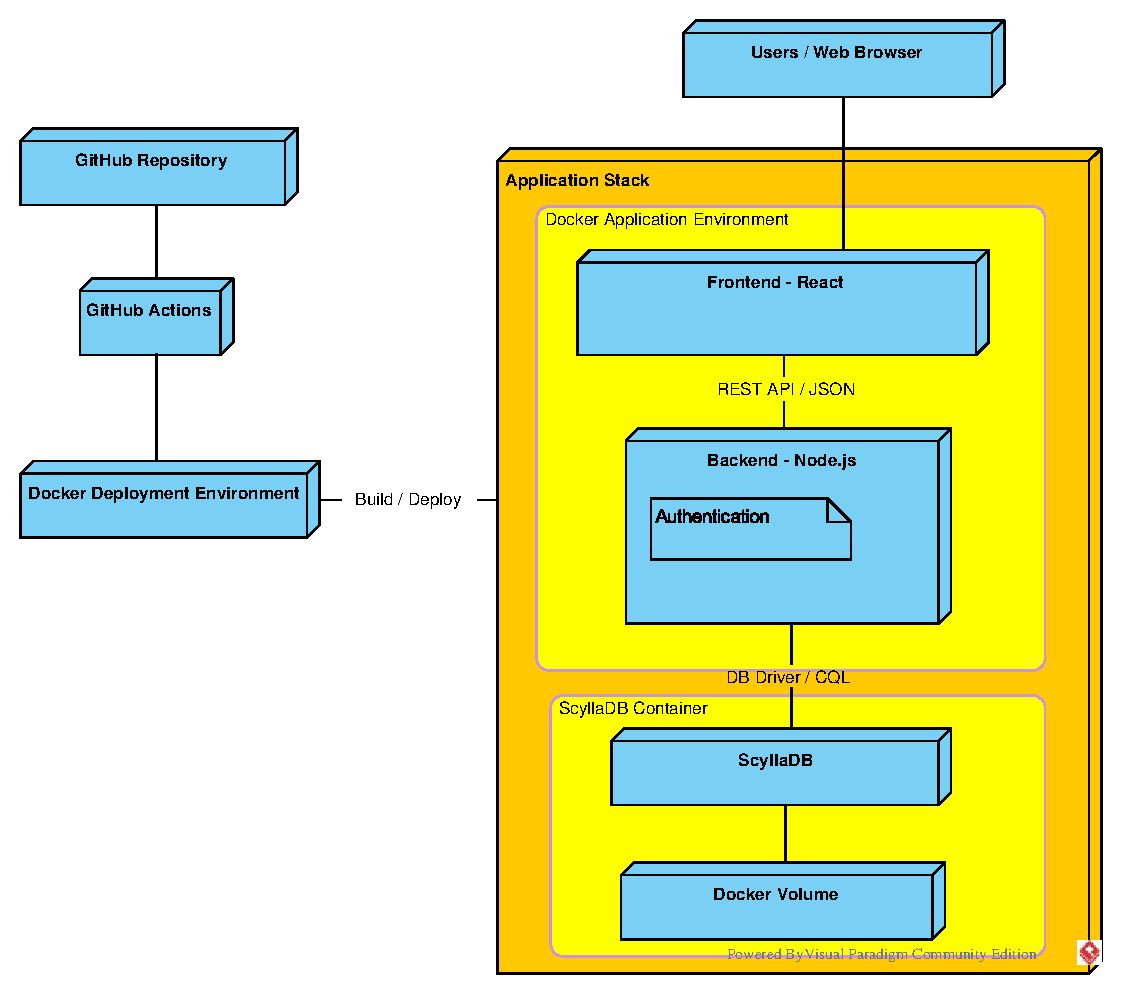
\includegraphics[width=0.88\textwidth]{eps/Deployment_Diagram1.eps}
    \caption{Dynamo technology stack.
    \label{Figure:TechnologyStackDiagram}}
\end{figure}
\index{Technology Stack Diagram}



\chapter{Use Cases}
\ChapterLabel{UseCases}
%\section{How to Use This Chapter}
%Describe goal-oriented interactions at the system boundary. Give every use case
%a stable ID, its own table, and at least one reciprocal requirement mapping.
%Include preconditions, trigger, main flow, alternate or exception flows, and
%postconditions. Maintain the canonical relationships among stories,
%requirements, use cases, and tests in \ChapterRef{Traceability}.

% \section[High-Level Use Case Diagram]{\hspace{0.5em}High-Level Use Case Diagram}
% Show the system boundary, primary actors, and major user goals before the
% detailed use-case tables. Replace the generic example with project-specific
% actors and use cases while preserving the stable use-case identifiers.

\begin{figure}[h]
\centering
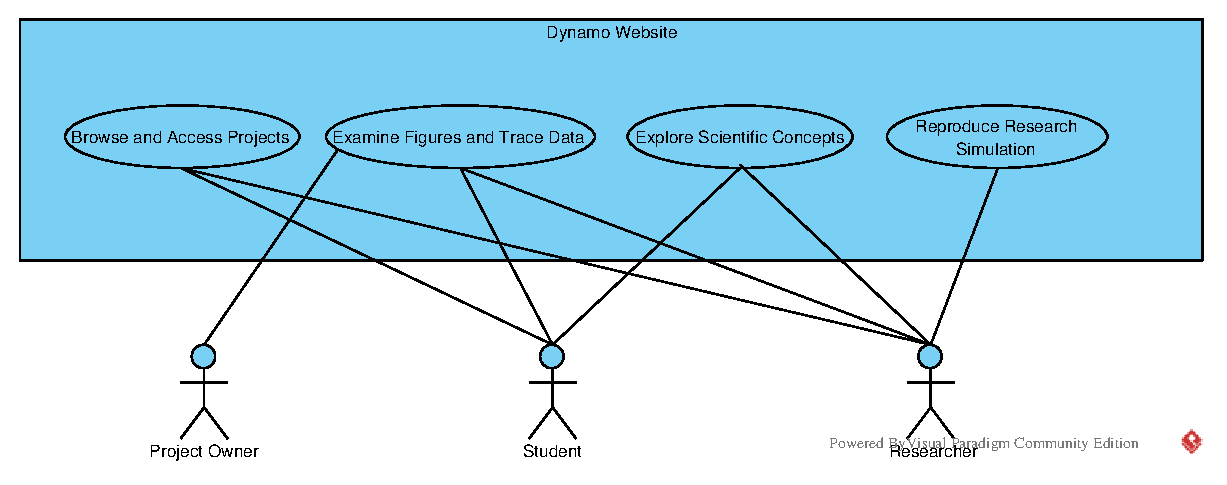
\includegraphics[width=0.88\textwidth]{eps/dsnUseCases/Dynamo_Diagram.eps}
\caption{Dynamo website use case diagram.\label{Figure:UseCaseDiagram}}
\end{figure}
\index{use case diagram}

\section{Browse and Access Research Projects}
\begin{tabularx}{\linewidth}{L{3.5cm}Y}
\toprule
\textbf{Identifier} & \UseCaseID{UC-001}\\
\textbf{Mapped requirements} & \RequirementRef{REQ-B-001}, \RequirementRef{REQ-Q-003}, \RequirementRef{REQ-Q-004}, \RequirementRef{REQ-Q-005}, \RequirementRef{REQ-S-004}, \RequirementRef{REQ-C-001}, \RequirementRef{REQ-C-003}\\
\textbf{Goal} & Allow users to find and access research papers, simulation code, datasets, and other research artifacts associated with a project.\\
\textbf{Primary actor} & Researcher, Student, or General Public\\
\textbf{Preconditions} & The website is accessible through a supported web browser and the requested research project exists on the platform.\\
\textbf{Trigger} & The user selects a research project from the website.\\
\textbf{Main flow} & The user browses or searches for a research project; the system displays the project overview and available research artifacts; the user selects an artifact; and the system retrieves and displays the selected artifact while distinguishing raw simulation output from processed or analyzed data.\\
\textbf{Alternate flow} & If the requested project or artifact does not exist, the system informs the user that no matching resource was found.\\
\textbf{Postconditions} & The selected research project or artifact has been displayed to the user without modifying the stored artifact.\\
\bottomrule
\end{tabularx}

\section{Explore Scientific Concepts}
\begin{tabularx}{\linewidth}{L{3.5cm}Y}
\toprule
\textbf{Identifier} & \UseCaseID{UC-002}\\
\textbf{Mapped requirements} & \RequirementRef{REQ-B-003}, \RequirementRef{REQ-F-001}, \RequirementRef{REQ-C-001}\\
\textbf{Goal} & Allow users to understand fundamental scientific concepts, variables, physical definitions, and units relevant to a research project.\\
\textbf{Primary actor} & Student, Researcher, or General Public\\
\textbf{Preconditions} & The research project contains documented scientific concepts or definitions.\\
\textbf{Trigger} & The user selects a scientific concept or definition associated with the research project.\\
\textbf{Main flow} & The user opens the project's concept documentation; the system displays an explanation of the selected concept; the system displays relevant scientific variables, physical definitions, and units; and the user reviews the information.\\
\textbf{Alternate flow} & If the selected concept does not have available documentation, the system informs the user that the concept has not yet been documented.\\
\textbf{Postconditions} & The user has access to the available explanation and definitions for the selected scientific concept.\\
\bottomrule
\end{tabularx}


\section{Examine Figures and Trace Supporting Data}
\begin{tabularx}{\linewidth}{L{3.5cm}Y}
\toprule
\textbf{Identifier} & \UseCaseID{UC-003}\\
\textbf{Mapped requirements} & \RequirementRef{REQ-B-004}, \RequirementRef{REQ-D-005}, \RequirementRef{REQ-C-001}\\
\textbf{Goal} & Allow users to understand key research figures and trace the figures back to the supporting data, analysis procedures, and simulation parameters.\\
\textbf{Primary actor} & Researcher, Third-Party Researcher, or General Public\\
\textbf{Preconditions} & The research project contains at least one documented figure and associated research data.\\
\textbf{Trigger} & The user selects a research figure.\\
\textbf{Main flow} & The user selects a figure; the system displays an explanation of the figure and its relationship to the research; the system displays the quantities and units represented by the figure; the system identifies the supporting data and processing or analysis procedure; and the system provides links to the relevant simulation parameters and source data.\\
\textbf{Alternate flow} & If supporting data or processing information is unavailable, the system displays the figure and available documentation while indicating which supporting information is unavailable.\\
\textbf{Postconditions} & The user can identify the relationship between the figure, supporting data, analysis procedure, and simulation parameters.\\
\bottomrule
\end{tabularx}


\section{Reproduce Results}
\begin{tabularx}{\linewidth}{L{3.5cm}Y}
\toprule
\textbf{Identifier} & \UseCaseID{UC-004}\\
\textbf{Mapped requirements} & \RequirementRef{REQ-B-005}, \RequirementRef{REQ-D-004}, \RequirementRef{REQ-D-005}, \RequirementRef{REQ-D-006}, \RequirementRef{REQ-C-001}\\
\textbf{Goal} & Provide a researcher with sufficient data, metadata, and procedures to reproduce a documented simulation and its associated analysis.\\
\textbf{Primary actor} & Researcher or Third-Party Researcher\\
\textbf{Preconditions} & The research project contains thorough instructions for reproducing results. \\
\textbf{Trigger} & The researcher selects a simulation and chooses to review its reproduction information.\\
\textbf{Main flow} & The researcher finds a project; a docker image and documentation are provided;\\
\textbf{Alternate flow} & If required reproduction information is missing, the system identifies the unavailable information and informs the researcher that the simulation cannot be fully reproduced from the available documentation.\\
\textbf{Postconditions} & The researcher has access to the available simulation inputs, metadata, data, and analysis procedures needed for reproduction.\\
\bottomrule
\end{tabularx}


\section{Manage Research Artifacts}
\begin{tabularx}{\linewidth}{L{3.5cm}Y}
\toprule
\textbf{Identifier} & \UseCaseID{UC-005}\\
\textbf{Mapped requirements} & \RequirementRef{REQ-F-003}, \RequirementRef{REQ-Q-001}, \RequirementRef{REQ-Q-002}, \RequirementRef{REQ-Q-003}, \RequirementRef{REQ-Q-005}, \RequirementRef{REQ-I-001}, \RequirementRef{REQ-I-002}, \RequirementRef{REQ-S-001}, \RequirementRef{REQ-S-002}, \RequirementRef{REQ-S-003}, \RequirementRef{REQ-S-005}, \RequirementRef{REQ-D-001}, \RequirementRef{REQ-D-004}, \RequirementRef{REQ-D-005}, \RequirementRef{REQ-D-006}, \RequirementRef{REQ-D-008}, \RequirementRef{REQ-C-001}, \RequirementRef{REQ-C-002}, \RequirementRef{REQ-C-003}\\
\textbf{Goal} & Allow authorized researchers to upload, edit, and manage research artifacts while maintaining version history and provenance.\\
\textbf{Primary actor} & Researcher or Project Owner\\
\textbf{Preconditions} & The researcher is authenticated and has appropriate permissions for the research project.\\
\textbf{Trigger} & The researcher chooses to upload or modify a research artifact.\\
\textbf{Main flow} & The researcher logs into their account; the system verifies the researcher's credentials; the researcher uploads or modifies an artifact such as code, data, images, videos, or a Docker image; the system stores the artifact without modifying its contents; the system records relevant metadata and provenance; and the system creates a timestamped version-history entry.\\
\textbf{Alternate flow} & If the researcher is not authenticated or does not have the required permissions, the system denies the requested modification. If the uploaded artifact is invalid or cannot be stored, the system reports the error and does not create the new version.\\
\textbf{Postconditions} & The authorized artifact has been stored or updated, and the modification is recorded in the artifact's version history and provenance information.\\
\bottomrule
\end{tabularx}


\section{Review Experiment History and Results}
\begin{tabularx}{\linewidth}{L{3.5cm}Y}
\toprule
\textbf{Identifier} & \UseCaseID{UC-007}\\
\textbf{Mapped requirements} & \RequirementRef{REQ-B-002}, \RequirementRef{REQ-F-002}, \RequirementRef{REQ-D-003}, \RequirementRef{REQ-D-004}, \RequirementRef{REQ-C-001}\\
\textbf{Goal} & Allow researchers to review experiments conducted for a project and examine the associated parameters and results.\\
\textbf{Primary actor} & Researcher or Third-Party Researcher\\
\textbf{Preconditions} & The research project contains a record of one or more experiments.\\
\textbf{Trigger} & The user opens the experiment history for a research project.\\
\textbf{Main flow} & The user selects a research project; the system displays the experiment log; the user selects an experiment; the system displays the experiment's initial conditions, input parameters, output dataset identifier, and relevant metadata; and the system allows results from different accretion disk scale heights to be compared.\\
\textbf{Alternate flow} & If an experiment does not contain complete result information, the system displays the available information and identifies missing data or metadata.\\
\textbf{Postconditions} & The user has reviewed the available experiment history and results, including the parameters associated with the selected experiment.\\
\bottomrule
\end{tabularx}


\section{Manage Collaboration and Access}
\begin{tabularx}{\linewidth}{L{3.5cm}Y}
\toprule
\textbf{Identifier} & \UseCaseID{UC-008}\\
\textbf{Mapped requirements} & \RequirementRef{REQ-S-002}, \RequirementRef{REQ-C-001}\\
\textbf{Goal} & Allow project owners to control collaborator access to research materials and maintain a record of modifications.\\
\textbf{Primary actor} & Researcher or Project Owner\\
\textbf{Preconditions} & The project owner is authenticated and has permission to manage access for the research project.\\
\textbf{Trigger} & The project owner chooses to add, modify, or remove a collaborator's edit access.\\
\textbf{Main flow} & The project owner selects a research project; the system displays current collaborators and their permissions; the project owner grants or removes edit access; the system verifies the owner's authorization; and the system records subsequent authorized modifications with the responsible user and timestamp.\\
\textbf{Alternate flow} & If the requesting user is not authorized to manage project access, the system denies the access-management request. If a collaborator does not have edit permission, the system prevents that collaborator from modifying the associated research material.\\
\textbf{Postconditions} & The project's collaborator permissions reflect the authorized changes, and modifications to research artifacts remain traceable to the responsible user and timestamp.\\
\bottomrule
\end{tabularx}

\section{Register a Published Paper Using a DOI}
\begin{tabularx}{\linewidth}{L{3.5cm}Y}
\toprule
\textbf{Identifier} & \UseCaseID{UC-009}\\
\textbf{Mapped requirements} & \RequirementRef{REQ-F-003}, \RequirementRef{REQ-D-007}, \RequirementRef{REQ-C-001}\\
\textbf{Goal} & Allow a researcher to register an existing publication by DOI and automatically populate its bibliographic information.\\
\textbf{Primary actor} & Researcher or Project Owner\\
\textbf{Preconditions} & The researcher is logged in on an account, the paper they are finding by DOI is published in a journal.\\
\textbf{Trigger} & The researcher chooses to add an existing publication using its DOI.\\
\textbf{Main flow} & The researcher enters a DOI; the system validates its format and requests available publication metadata from a DOI metadata provider; the system displays the retrieved title, authors, publication date, and source for confirmation; the researcher confirms or corrects the information; and the system associates the publication record with the research project.\\
\textbf{Alternate flow} & If the DOI is invalid, not found, or the metadata provider is unavailable, the system reports the problem and allows the researcher to retry or enter the bibliographic details manually. If the researcher lacks permission, the system refuses to modify the project.\\
\textbf{Postconditions} & A confirmed publication record is associated with the project; the DOI identifies the external publication and does not imply that its full text was uploaded.\\
\bottomrule
\end{tabularx}

\section{Making an Account}
\begin{tabularx}{\linewidth}{L{3.5cm}Y}
\toprule
\textbf{Identifier} & \UseCaseID{UC-010}\\
\textbf{Mapped requirements} & \RequirementRef{REQ-F-003}, \RequirementRef{REQ-D-007}, \RequirementRef{REQ-C-001}\\
\textbf{Goal} & Allow a researcher create an account that will enable them to upload work.\\
\textbf{Primary actor} & Researcher or Project Owner\\
\textbf{Preconditions} & The researcher has an email account. \\
\textbf{Trigger} & The researcher clicks the sign up button. \\
\textbf{Main flow} & The researcher enters a username, email, and password. There will also be a field to confirm the password. After the researcher clicks sign up, a verification email is sent to the email. After the link in the email is clicked on, the account is verified and created.\\
\textbf{Alternate flow} & If the link in the verification email is not clicked on, the account is unverified and not created. \\
\textbf{Postconditions} & The researcher has an account on the platform. \\
\bottomrule
\end{tabularx}

\section{Uploading a Paper Directly}
\begin{tabularx}{\linewidth}{L{3.5cm}Y}
\toprule
\textbf{Identifier} & \UseCaseID{UC-010}\\
\textbf{Mapped requirements} & \RequirementRef{REQ-F-003}, \RequirementRef{REQ-D-007}, \RequirementRef{REQ-C-001}\\
\textbf{Goal} & Allow a researcher to upload their work even if its paywalled.\\
\textbf{Primary actor} & Researcher or Project Owner\\
\textbf{Preconditions} & The paper is published in a journal.\\
\textbf{Trigger} & The researcher chooses to add an existing publication by uploading a pdf.\\
\textbf{Main flow} & The researcher uploads a pdf of their paper from their device. The platform verifies that the paper is published in a journal and that one of the authors' emails listed in the paper is associated with the account of the researcher. The platform validates the pdf format and
requests available publication metadata from a DOI metadata
provider; the platform displays the retrieved title, authors, publication
date, and source for confirmation; the researcher confirms or corrects
the information; and the system associates the paper with the research project.\\
\textbf{Alternate flow} & If none of the emails are associated with the account owner, the upload is denied.\\
\textbf{Postconditions} & The paper is now uploaded on the platform. \\
\bottomrule
\end{tabularx}
%\chapter{Architecture Overview}
\ChapterLabel{ArchitectureOverview}
\section{How to Use This Chapter}
Explain the forces that shape the design, the major decisions, alternatives considered, and consequences. Use the 4+1 views only when they help readers answer different architectural questions.
\section{Decision Template and Example}
\textbf{ARC-001:} \textit{[Decision]}; \textbf{Drivers:} \textit{[quality attributes and constraints]}; \textbf{Rationale:} \textit{[why selected]}; \textbf{Consequences:} \textit{[benefits, trade-offs, and risks]}. Example: use an asynchronous message queue to protect request processing from transient downstream outages; this improves resilience but introduces eventual consistency.

%\chapter{User Interface Design}
\ChapterLabel{UserInterfaceDesign}
\section{How to Use This Chapter}
Describe personas, primary screens or workflows, interaction rules, feedback, accessibility, and essential states. Include wireframes or prototypes where they resolve meaningful ambiguity.
\section{Example}
Persona: a busy operations coordinator needs to submit and track requests quickly. The request screen groups required fields, identifies inline validation errors, confirms successful submission, supports keyboard operation, and exposes empty, loading, error, and completed states.

%\chapter{Logical View}
\ChapterLabel{LogicalView}
\section{How to Use This Chapter}
Model the domain concepts, responsibilities, relationships, data ownership, and invariants without committing to code-level structure. Use a class, entity, or conceptual diagram where useful.
\section{Example}
\textit{Request} has an identifier, submitter, status, and submitted time. A request has one or more \textit{Request Items}. Invariants: every identifier is unique; every request has a valid status; an approved request cannot return to Draft without an authorized transition.

%\chapter{Process View}
\ChapterLabel{ProcessView}
\section{How to Use This Chapter}
Describe runtime behavior, concurrency, state transitions, workflows, error handling, and significant sequences. Use activity, sequence, or state diagrams when prose is insufficient.
\section{Example State Model}
Request states are Draft, Submitted, Under Review, Approved, Rejected, and Cancelled. Submission moves Draft to Submitted only when required data is valid. Approval and rejection are terminal except for an authorized correction workflow.

%\chapter{Development View}
\ChapterLabel{DevelopmentView}
\section{How to Use This Chapter}
Show how source code, modules, services, libraries, and build artifacts are organized. State dependency rules so that implementers do not create forbidden coupling.
\section{Example}
Organize a service into presentation/API, application workflow, domain model, and infrastructure adapters. The API calls application services; application services depend on domain abstractions; infrastructure implements those abstractions. Domain logic must not depend on the web framework or database driver.

%\chapter{Physical View}
\ChapterLabel{PhysicalView}
\section{How to Use This Chapter}
Describe deployment nodes, networks, environments, runtime dependencies, trust boundaries, data stores, and operations constraints. Include a deployment diagram for distributed systems.
\section{Example}
A browser communicates over TLS with an API service. The API service uses a private database network; backups are encrypted and access is limited to the operations role. Define availability targets, monitoring, and recovery responsibilities.


%\chapter{Constraints and Assumptions}\ChapterLabel{ConstraintsAssumptions}
%\section{Design and Implementation Constraints}
%Record mandated technologies, budgets, schedules, standards, interfaces, facilities, safety limits, and other restrictions.
%\section{Assumptions and Dependencies}
%Record assumptions, external dependencies, owners, risks if invalidated, and contingency plans.

%\chapter{Applicable Codes, Standards, and Regulations}\ChapterLabel{CodesStandardsRegulations}
%Identify the applicable codes, standards, regulations, policies, and ethical obligations. State how the project will demonstrate compliance.

%\chapter{Concept Development and Selection}\ChapterLabel{ConceptDevelopment}
%Document alternatives, screening criteria, trade studies, stakeholder input, concept selection rationale, and the resulting baseline concept.

%\begin{dsnMilestone}[Milestone 1: Design Proposal]
%First week of October: present the mission, customer, needs, requirements, and concepts.
%\end{dsnMilestone}

%\chapter{Preliminary and Detailed Design}\ChapterLabel{PreliminaryDetailedDesign}
%Document geometry, materials, manufacturing alternatives, software/hardware decomposition, and system-integration plans.
%\section{System Architecture}
%\subsection{Overview of System Architecture}
%Show the system boundary, major subsystems, data/material/energy flows, responsibilities, and integration strategy.
%\subsection{Hardware Architecture}
%Describe hardware subsystems, interfaces, and allocation of requirements.
%\subsection{Software Architecture}
%Describe software layers, components, data flows, deployment, and allocation of requirements.
%\subsection{Security Architecture}
%Describe assets, threats, trust boundaries, controls, access rules, and residual risks as applicable.
%\subsection{Communication Architecture}
%Describe protocols, networks, message/data formats, timing, and failure handling.
%\section{System Design}
%\subsection{System Behavior Description}
%Describe system states, workflows, use cases, timing, error handling, and safety behavior.
%\subsection{Databases/Data Storage}
%Describe data models, data lifecycle, retention, backup, privacy, and integrity controls.
%\subsection{Data Conversion}
%Describe imported, transformed, migrated, or exported data and its validation.
%\subsection{Sub-System Interfaces}
%Specify interfaces, signals, protocols, APIs, tolerances, and integration responsibilities.
%\subsection{User Interface Design}
%Present user tasks, wireframes, interaction flows, accessibility considerations, and usability criteria.
%\section{Mechanical Design}
%\subsection{Components and Sub-Assemblies - Bill of Materials}
%Provide the bill of materials, part identifiers, quantities, sources, costs, and assembly relationships.
%\subsection{Geometric Specification - CAD Models/Drawings}
%Provide or reference controlled CAD models, drawings, dimensions, tolerances, and revision identifiers.
%\subsection{Materials Selected}
%Justify material selections using relevant mechanical, environmental, cost, and safety criteria.
%\subsection{Manufacturing Processes Selected}
%Describe selected processes, capabilities, quality controls, and alternatives considered.
%\subsection{Process Description or Optimization Notes}
%Document process steps, parameters, optimization results, and lessons learned.
%\section{Electronics/Electro-Mechanical Design}
%\subsection{Circuits}
%Provide schematics, circuit rationale, design calculations, and test points.
%\subsection{Electrical and Electro-Mechanical Interfaces}
%Specify connectors, signals, power, mechanical mounting, protections, and interface constraints.
%\subsection{List of Components: Motors, Sensors, Electronics}
%List components, part numbers, specifications, source, cost, and selection rationale.
%\subsection{Power System}
%Describe power sources, budgets, conversion, distribution, protection, battery charging, and safety.
%\section{Software Components Design}
%\subsection{Algorithms}
%Describe algorithms, inputs, outputs, assumptions, complexity/performance, and validation approach.
%\subsection{Modules/Classes/Methods}
%Describe modules, classes, methods, responsibilities, dependencies, and interfaces.
%\subsection{Application Programming Interfaces}
%Specify APIs, endpoints, contracts, error behavior, versioning, and authentication as applicable.
%\subsection{Coding/Implementation Details}
%Describe key implementation decisions, build/run process, configuration, and coding conventions.

%\chapter{Design Evaluation Methods}\ChapterLabel{DesignEvaluationMethods}
%\section{Design Concepts and Concept Screening}
%Update concept screening if the alternatives or criteria changed after the initial selection.
%\section{Design Evaluation/Selection Methods}
%Describe the evaluation method, metrics, weights, experimental design, analysis technique, and decision rule.
%\section{Analysis Cases and Results}
%Present analysis cases, assumptions, calculations, simulation or experiment results, uncertainty, and conclusions.
%\section{Impact on System Design}
%Explain how analysis results determined system parameters and resulting design revisions.

%\begin{dsnMilestone}[Milestone 2: Preliminary Design Review]
%Third week of November: document the design, finalized concept evaluation and selection, and analysis.
%\end{dsnMilestone}

%\chapter{Alpha Prototyping: Plan and Budget}\ChapterLabel{AlphaPrototyping}
%Define the alpha prototype scope, integration plan, demonstration criteria, budget, procurement, and test plan. The alpha demonstration must show all components and subsystems and how they fit together; full system integration is not required, but every individual subsystem must function.

%\chapter{Testing and Evaluation: Plan and Results}\ChapterLabel{TestingEvaluation}
%Provide test objectives, procedures, equipment, data, pass/fail criteria, results, anomalies, corrective actions, and traceability to requirements.

%\chapter{Tests}
\ChapterLabel{Tests}
\section{Planned Test Cases}
The tests below are proposed verification procedures, not recorded execution results. Evidence, dates, environments, and actual pass/fail outcomes must be added after execution.
\small
\begin{longtable}{p{1.5cm}p{2.8cm}p{6.0cm}p{5.0cm}}
\caption{Planned Dynamo Test Cases\label{Table:TestCaseExamples}}\\
\toprule
\textbf{ID} & \textbf{Mapped requirement} & \textbf{Procedure} & \textbf{Expected result}\\
\midrule\endfirsthead
\toprule\textbf{ID} & \textbf{Mapped requirement} & \textbf{Procedure} & \textbf{Expected result}\\\midrule\endhead
\TestCaseID{TC-001} & \RequirementRef{REQ-D-001} & As an authorized researcher, upload a supported research artifact and provide metadata. & The artifact is saved, linked to the project, and can be retrieved.\\
\TestCaseID{TC-002} & \RequirementRef{REQ-Q-002} & Upload an artifact, then submit a modified version and inspect version history. & Two timestamped versions exist and the previous version remains accessible.\\
\TestCaseID{TC-003} & \RequirementRef{REQ-Q-003} & Upload a known binary file, retrieve it, and compare cryptographic hashes. & Uploaded and retrieved file hashes match.\\
\TestCaseID{TC-004} & \RequirementRef{REQ-S-002} & Attempt to edit an artifact as an authorized whitelisted user and a non-whitelisted user. & The authorized edit succeeds; the unauthorized edit is denied.\\
\TestCaseID{TC-005} & \RequirementRef{REQ-D-007} & Enter a known valid DOI and inspect fetched bibliographic metadata. & Available title and author information is populated and can be confirmed before saving.\\
\TestCaseID{TC-006} & \RequirementRef{REQ-F-003} & Register a published paper within a research project and retrieve its record. & The paper record is accessible from the project.\\
\TestCaseID{TC-007} & \RequirementRef{REQ-D-008} & Upload files at the approved 1 GB limit and above the limit. & The at-limit upload is accepted subject to system resources; larger uploads are rejected.\\
\TestCaseID{TC-008} & \RequirementRef{REQ-C-001} & Run core use-case tests in every approved browser and deployment environment. & Core workflows operate in the approved baseline.\\
\TestCaseID{TC-009} & \RequirementRef{REQ-B-001} & Open a published project as a public visitor and inspect available artifacts. & The research paper and any publicly shared datasets or code are accessible.\\
\TestCaseID{TC-010} & \RequirementRef{REQ-Q-001} & Ask a researcher without programming expertise to upload and manage an artifact using the browser. & The researcher completes the workflow without writing code.\\
\TestCaseID{TC-011} & \RequirementRef{REQ-D-006} & Use the documented inputs, parameters, code, and environment to attempt reproduction. & The required reproduction materials can be located; any missing materials are reported.\\
\TestCaseID{TC-012} & \RequirementRef{REQ-C-002} & Access the artifact-management workflow using a browser on a machine without developer tools. & The workflow runs without installing native software.\\
\TestCaseID{TC-013} & \RequirementRef{REQ-C-003} & Run the critical project tasks across every approved OS and browser combination. & Core tasks are available across the approved combinations.\\
\TestCaseID{TC-014} & \RequirementRef{REQ-B-002} & Open an experiment log and review run parameters and recorded outputs. & Runs, associated parameters, and results are accessible.\\
\TestCaseID{TC-015} & \RequirementRef{REQ-B-003} & Open a documented scientific concept and inspect its definitions and units. & The corresponding explanations, variables, and units are displayed.\\
\TestCaseID{TC-016} & \RequirementRef{REQ-B-004} & Select a research figure and inspect its data and analysis links. & The figure and its supporting sources or explicit missing-data notices appear.\\
\TestCaseID{TC-017} & \RequirementRef{REQ-B-005} & Select reproduction guidance for a published result. & Available simulation instructions and input references are displayed.\\
\TestCaseID{TC-018} & \RequirementRef{REQ-F-001} & Open the concept wiki and select an entry. & The selected scientific concept is displayed.\\
\TestCaseID{TC-019} & \RequirementRef{REQ-F-002} & Open a project progress log and inspect entries. & Available research progress entries are displayed.\\
\TestCaseID{TC-020} & \RequirementRef{REQ-I-002} & Upload a supported research video and open it from the project view. & The video can be uploaded and displayed.\\
\TestCaseID{TC-021} & \RequirementRef{REQ-S-003} & Log in with valid credentials and then with an invalid password. & Only valid credentials establish an authenticated session.\\
\TestCaseID{TC-022} & \RequirementRef{REQ-S-004} & Visit a public paper page without signing in. & Public paper content is accessible without an account.\\
\TestCaseID{TC-023} & \RequirementRef{REQ-S-005} & Request a password recovery using a registered account. & The system supports a secure account-recovery flow.\\
\TestCaseID{TC-024} & \RequirementRef{REQ-Q-004} & Measure retrieval time of reference artifacts under the agreed test workload. & Each measured retrieval completes within five seconds.\\
\TestCaseID{TC-025} & \RequirementRef{REQ-Q-005} & Open project documentation independently of the original research-paper document. & Additional artifacts are accessible without changing the original paper.\\
\TestCaseID{TC-026} & \RequirementRef{REQ-D-003} & Inspect identifiers for datasets generated from distinct experiment parameters. & Output datasets have identifiers traceable to their generation parameters.\\
\TestCaseID{TC-027} & \RequirementRef{REQ-D-004} & Open the provenance record for a simulation dataset. & Software versions, configuration, and environment metadata are recorded.\\
\TestCaseID{TC-028} & \RequirementRef{REQ-D-005} & Trace a derived result to the data-processing procedure. & The applicable transformation and analysis procedures are available.\\
\TestCaseID{TC-029} & \RequirementRef{REQ-I-001} & Perform artifact creation and editing using only browser controls. & No coding or local software installation is necessary.\\
\TestCaseID{TC-030} & \RequirementRef{REQ-S-001} & Attempt create, edit, and delete operations with and without authorization. & Only authorized operations succeed.\\
\bottomrule
\end{longtable}
\normalsize

\chapter{Traceability}
\ChapterLabel{Traceability}
\index{traceability}
\index{requirements traceability matrix}
\section{How to Use This Chapter}
Maintain the canonical mapping from stakeholder need or approved constraint through requirement, design decision, implementation, test, verification, validation, and release evidence. Review both missing backward links and missing forward links.
\section{Traceability Register}
Requirement and use-case chapters contain reciprocal mappings. The verification and validation evidence columns remain blank until project-specific evidence is documented. An
unlinked requirement may be gold-plating; an untested requirement or unmapped
use case is incomplete.

\begin{landscape}
\small
\begin{tabularx}{\linewidth}{YYYYYY}
\caption{Traceability Register\label{Table:TraceabilityMatrix}}\\
\toprule
\textbf{User Story} & \textbf{Requirement} & \textbf{Use Case} & \textbf{Test Case} & \textbf{Verification} & \textbf{Validation}\\
\midrule
\endfirsthead
\multicolumn{6}{l}{\small\itshape Traceability Register (continued)}\\
\toprule
\textbf{User Story} & \textbf{Requirement} & \textbf{Use Case} & \textbf{Test Case} & \textbf{Verification} & \textbf{Validation}\\
\midrule
\endhead
\midrule
\multicolumn{6}{r}{\small\itshape Continued on next page}\\
\endfoot
\bottomrule
\endlastfoot
\UserStoryRef{US-001} & \RequirementRef{REQ-B-001} & \UseCaseRef{UC-001} & \TestCaseRef{TC-009} & -- & --\\
\UserStoryRef{US-016} & \RequirementRef{REQ-B-002} & \UseCaseRef{UC-007} & \TestCaseRef{TC-014} & -- & --\\
\UserStoryRef{US-003} & \RequirementRef{REQ-B-003} & \UseCaseRef{UC-002} & \TestCaseRef{TC-015} & -- & --\\
\UserStoryRef{US-003} & \RequirementRef{REQ-B-004} & \UseCaseRef{UC-003} & \TestCaseRef{TC-016} & -- & --\\
\UserStoryRef{US-004} & \RequirementRef{REQ-B-005} & \UseCaseRef{UC-004} & \TestCaseRef{TC-017} & -- & --\\
\UserStoryRef{US-002} & \RequirementRef{REQ-F-001} & \UseCaseRef{UC-002} & \TestCaseRef{TC-018} & -- & --\\
\UserStoryRef{US-016} & \RequirementRef{REQ-F-002} & \UseCaseRef{UC-007} & \TestCaseRef{TC-019} & -- & --\\
\UserStoryRef{US-020} & \RequirementRef{REQ-F-003} & \UseCaseRef{UC-005} & \TestCaseRef{TC-006} & -- & --\\
\UserStoryRef{US-020} & \RequirementRef{REQ-F-003} & \UseCaseRef{UC-009} & \TestCaseRef{TC-006} & -- & --\\
\UserStoryRef{US-008} & \RequirementRef{REQ-Q-001} & \UseCaseRef{UC-005} & \TestCaseRef{TC-010} & -- & --\\
\UserStoryRef{US-015} & \RequirementRef{REQ-Q-002} & \UseCaseRef{UC-005} & \TestCaseRef{TC-002} & -- & --\\
\UserStoryRef{US-001} & \RequirementRef{REQ-Q-003} & \UseCaseRef{UC-001} & \TestCaseRef{TC-003} & -- & --\\
\UserStoryRef{US-001} & \RequirementRef{REQ-Q-003} & \UseCaseRef{UC-005} & \TestCaseRef{TC-003} & -- & --\\
\UserStoryRef{US-001} & \RequirementRef{REQ-Q-004} & \UseCaseRef{UC-001} & \TestCaseRef{TC-024} & -- & --\\
\UserStoryRef{US-001} & \RequirementRef{REQ-Q-005} & \UseCaseRef{UC-001} & \TestCaseRef{TC-025} & -- & --\\
\UserStoryRef{US-001} & \RequirementRef{REQ-Q-005} & \UseCaseRef{UC-005} & \TestCaseRef{TC-025} & -- & --\\
\UserStoryRef{US-008} & \RequirementRef{REQ-I-001} & \UseCaseRef{UC-005} & \TestCaseRef{TC-029} & -- & --\\
\UserStoryRef{US-009} & \RequirementRef{REQ-I-002} & \UseCaseRef{UC-005} & \TestCaseRef{TC-020} & -- & --\\
\UserStoryRef{US-008} & \RequirementRef{REQ-S-001} & \UseCaseRef{UC-005} & \TestCaseRef{TC-030} & -- & --\\
\UserStoryRef{US-009} & \RequirementRef{REQ-S-002} & \UseCaseRef{UC-005} & \TestCaseRef{TC-004} & -- & --\\
\UserStoryRef{US-009} & \RequirementRef{REQ-S-002} & \UseCaseRef{UC-008} & \TestCaseRef{TC-004} & -- & --\\
\UserStoryRef{US-009} & \RequirementRef{REQ-S-003} & \UseCaseRef{UC-005} & \TestCaseRef{TC-021} & -- & --\\
\UserStoryRef{US-009} & \RequirementRef{REQ-S-004} & \UseCaseRef{UC-001} & \TestCaseRef{TC-022} & -- & --\\
\UserStoryRef{US-009} & \RequirementRef{REQ-S-005} & \UseCaseRef{UC-005} & \TestCaseRef{TC-023} & -- & --\\
\UserStoryRef{US-001} & \RequirementRef{REQ-D-001} & \UseCaseRef{UC-005} & \TestCaseRef{TC-001} & -- & --\\
\UserStoryRef{US-003} & \RequirementRef{REQ-D-003} & \UseCaseRef{UC-007} & \TestCaseRef{TC-026} & -- & --\\
\UserStoryRef{US-004} & \RequirementRef{REQ-D-004} & \UseCaseRef{UC-004} & \TestCaseRef{TC-027} & -- & --\\
\UserStoryRef{US-004} & \RequirementRef{REQ-D-004} & \UseCaseRef{UC-005} & \TestCaseRef{TC-027} & -- & --\\
\UserStoryRef{US-004} & \RequirementRef{REQ-D-004} & \UseCaseRef{UC-007} & \TestCaseRef{TC-027} & -- & --\\
\UserStoryRef{US-003} & \RequirementRef{REQ-D-005} & \UseCaseRef{UC-003} & \TestCaseRef{TC-028} & -- & --\\
\UserStoryRef{US-003} & \RequirementRef{REQ-D-005} & \UseCaseRef{UC-004} & \TestCaseRef{TC-028} & -- & --\\
\UserStoryRef{US-003} & \RequirementRef{REQ-D-005} & \UseCaseRef{UC-005} & \TestCaseRef{TC-028} & -- & --\\
\UserStoryRef{US-004} & \RequirementRef{REQ-D-006} & \UseCaseRef{UC-004} & \TestCaseRef{TC-011} & -- & --\\
\UserStoryRef{US-004} & \RequirementRef{REQ-D-006} & \UseCaseRef{UC-005} & \TestCaseRef{TC-011} & -- & --\\
\UserStoryRef{US-020} & \RequirementRef{REQ-D-007} & \UseCaseRef{UC-009} & \TestCaseRef{TC-005} & -- & --\\
\UserStoryRef{US-020} & \RequirementRef{REQ-D-008} & \UseCaseRef{UC-005} & \TestCaseRef{TC-007} & -- & --\\
\UserStoryRef{US-001} & \RequirementRef{REQ-C-001} & \UseCaseRef{UC-001} & \TestCaseRef{TC-008} & -- & --\\
\UserStoryRef{US-001} & \RequirementRef{REQ-C-001} & \UseCaseRef{UC-002} & \TestCaseRef{TC-008} & -- & --\\
\UserStoryRef{US-001} & \RequirementRef{REQ-C-001} & \UseCaseRef{UC-003} & \TestCaseRef{TC-008} & -- & --\\
\UserStoryRef{US-001} & \RequirementRef{REQ-C-001} & \UseCaseRef{UC-004} & \TestCaseRef{TC-008} & -- & --\\
\UserStoryRef{US-001} & \RequirementRef{REQ-C-001} & \UseCaseRef{UC-005} & \TestCaseRef{TC-008} & -- & --\\
\UserStoryRef{US-001} & \RequirementRef{REQ-C-001} & \UseCaseRef{UC-007} & \TestCaseRef{TC-008} & -- & --\\
\UserStoryRef{US-001} & \RequirementRef{REQ-C-001} & \UseCaseRef{UC-008} & \TestCaseRef{TC-008} & -- & --\\
\UserStoryRef{US-001} & \RequirementRef{REQ-C-001} & \UseCaseRef{UC-009} & \TestCaseRef{TC-008} & -- & --\\
\UserStoryRef{US-008} & \RequirementRef{REQ-C-002} & \UseCaseRef{UC-005} & \TestCaseRef{TC-012} & -- & --\\
\UserStoryRef{US-018} & \RequirementRef{REQ-C-003} & \UseCaseRef{UC-001} & \TestCaseRef{TC-013} & -- & --\\
\UserStoryRef{US-018} & \RequirementRef{REQ-C-003} & \UseCaseRef{UC-005} & \TestCaseRef{TC-013} & -- & --\\
\end{tabularx}
\end{landscape}

\chapter{Diagrams}
\ChapterLabel{Diagrams}

\section{Browse and Access Research Projects}

This diagram explains the search interaction supporting
\RequirementRef{REQ-Q-006}
and \RequirementRef{REQ-Q-009}.

\begin{figure}[h!]
\centering
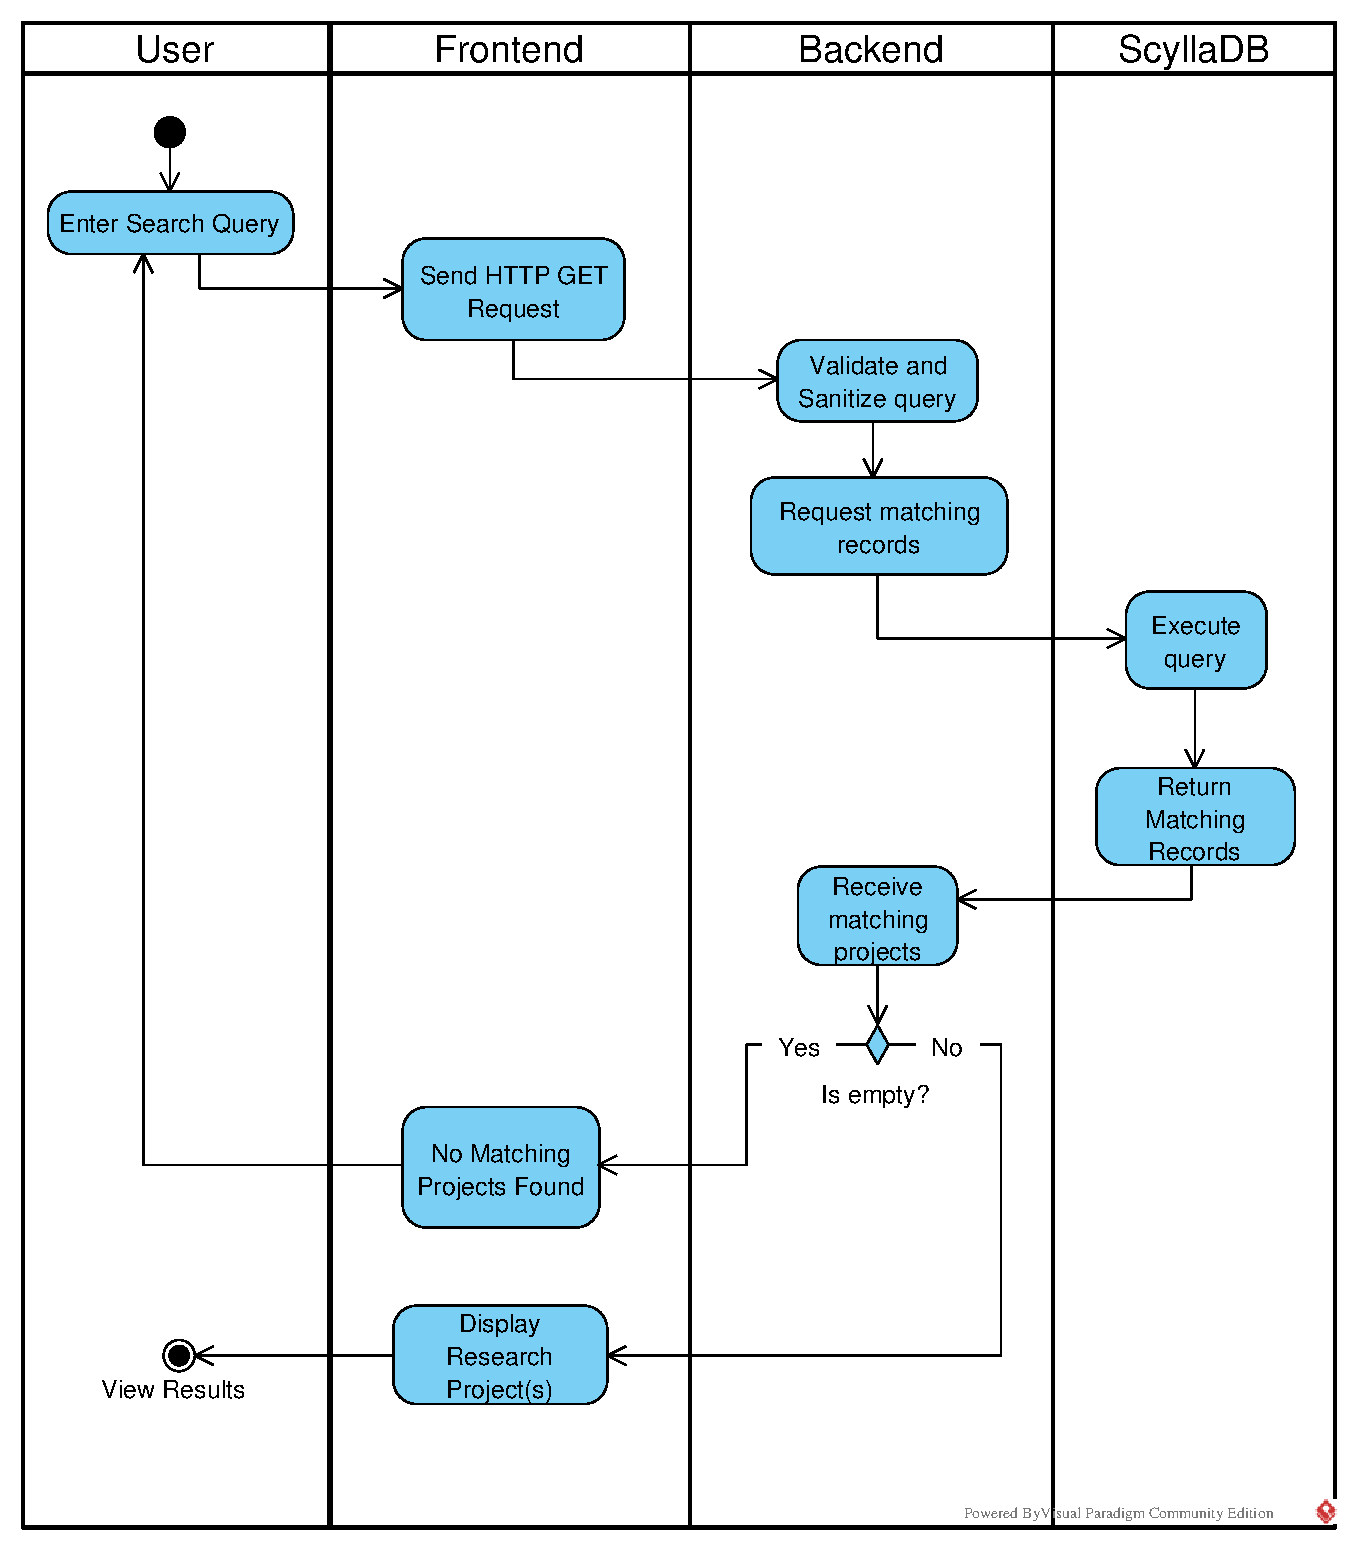
\includegraphics[width=0.65\textwidth]{diagrams/dsnUseCases/Swimlane.eps}
\caption{Search Function Sequence Diagram}
\label{Figure:SearchSequenceDiagram}
\end{figure}

\clearpage


\section{Manage Collaboration and Access}

The permission-management activity supports
\RequirementRef{REQ-S-001},
\RequirementRef{REQ-S-002}, and
\RequirementRef{REQ-F-005}.

\begin{figure}[h!]
\centering
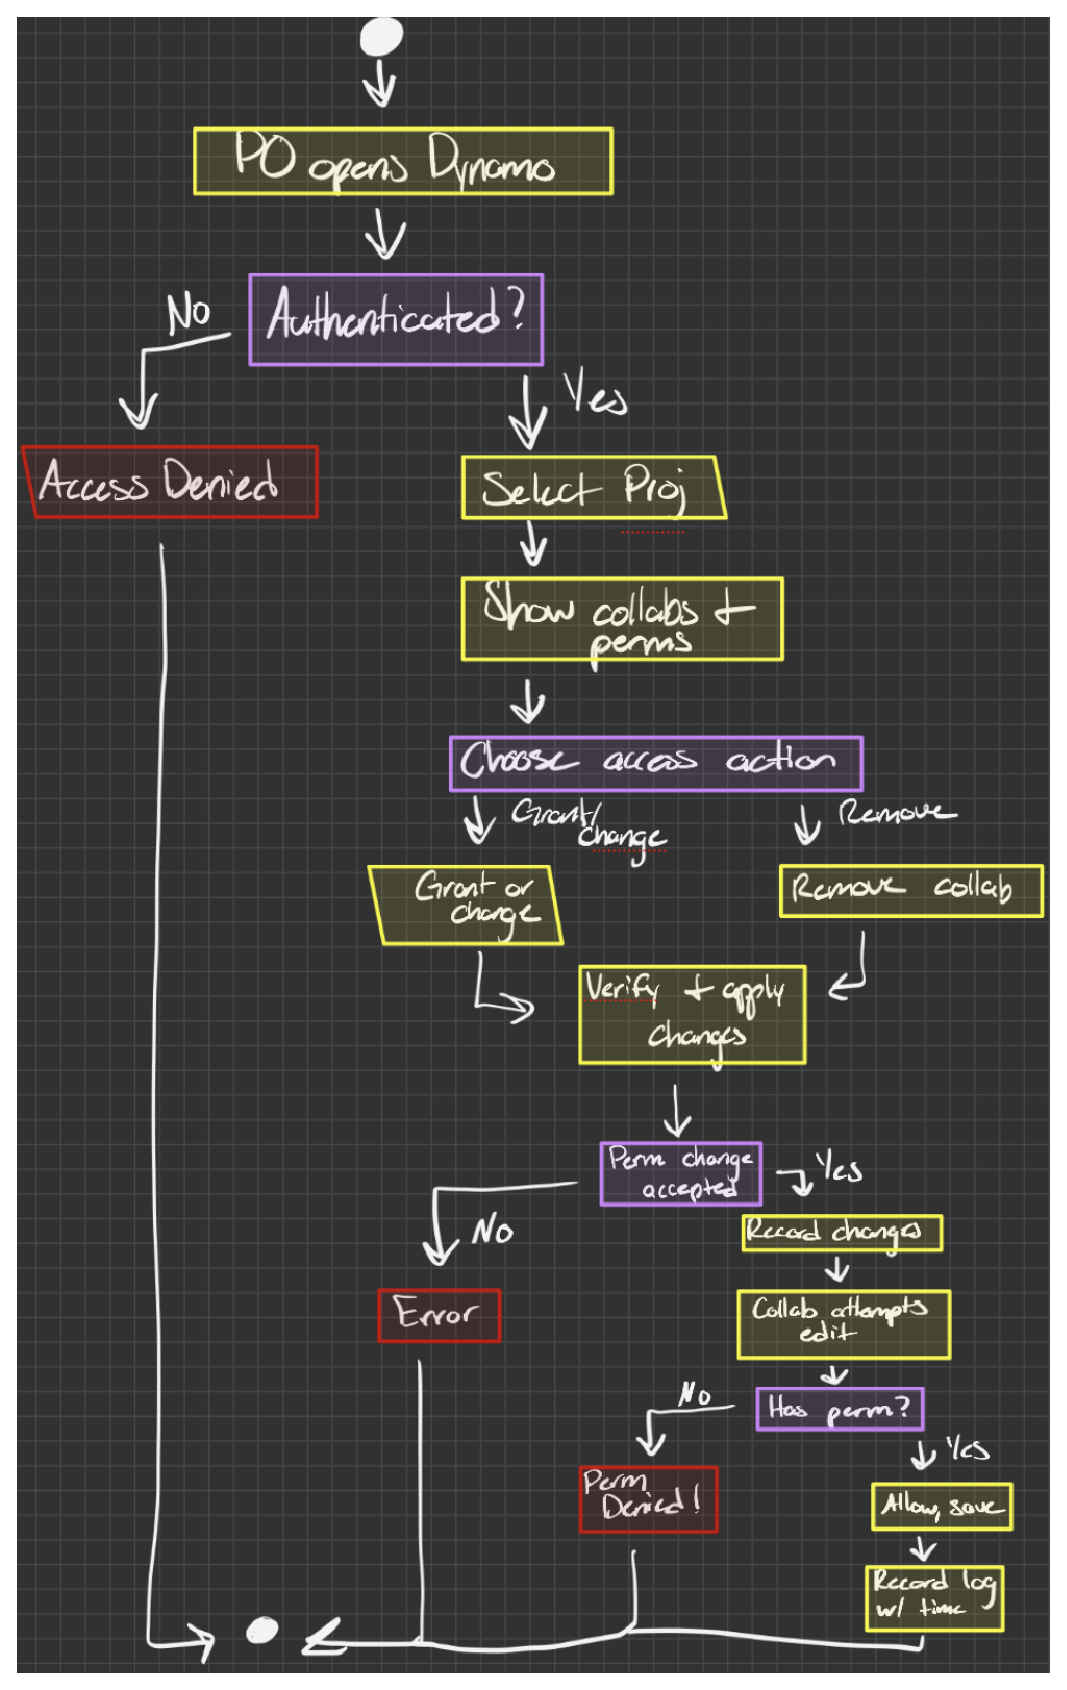
\includegraphics[width=0.5\textwidth]{eps/dsnUseCases/ManageCollaborationAndAccessActivityDiagram.eps}
\caption{Manage Collaboration And Access Use Case Diagram. \label{Figure:ManageCollaborationAndAccessUseCaseDiagram}}
\end{figure}
\index{use case diagram}

\clearpage

\section{Register a Published Paper Using a DOI}

Supports
\RequirementRef{REQ-F-003},
\RequirementRef{REQ-F-004},
\RequirementRef{REQ-F-005}, and
\RequirementRef{REQ-D-007}.

\begin{figure}[h!]
\centering
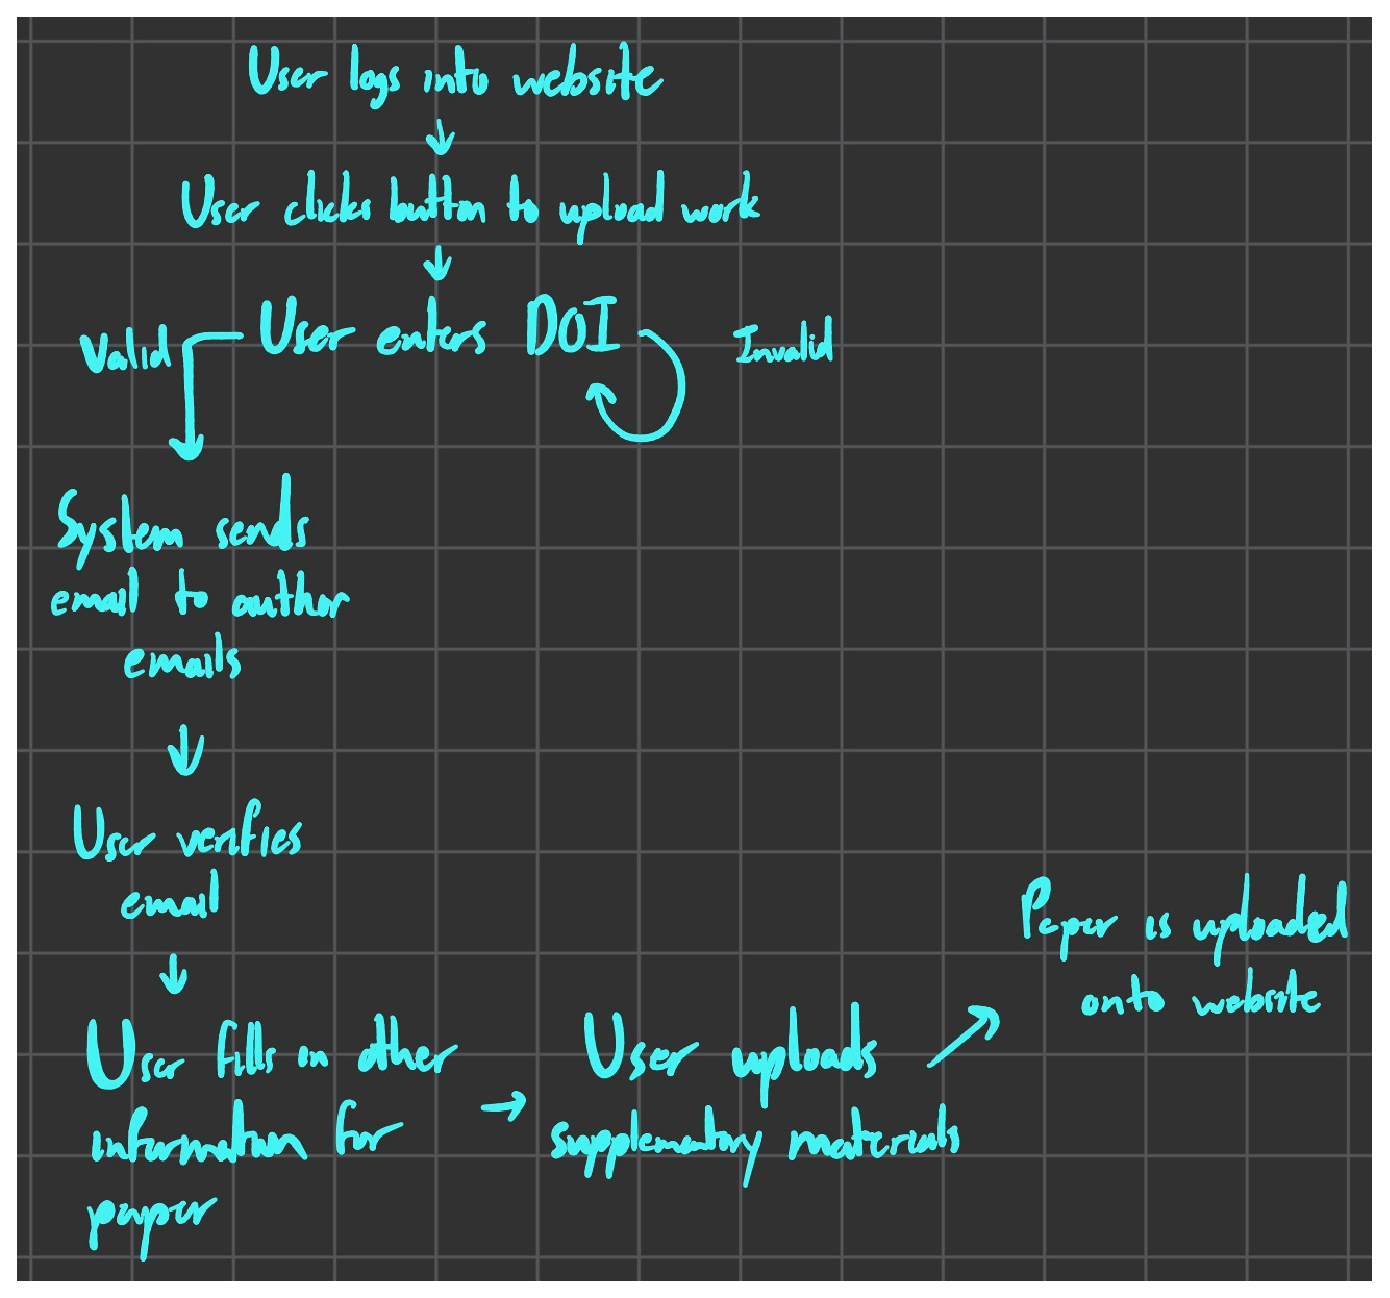
\includegraphics[width=0.5\textwidth]{eps/dsnUseCases/UploadDocumentActivityDiagram.eps}
\caption{Register a Published Paper Using a DOI Use Case Diagram.\label{Figure:DOIUploadUseCaseDiagram}}
\end{figure}
\index{use case diagram}

\clearpage

\section{Manage Research Artifacts}

This workflow supports
\RequirementRef{REQ-D-001},
\RequirementRef{REQ-Q-001},
\RequirementRef{REQ-Q-002},
\RequirementRef{REQ-Q-003},
\RequirementRef{REQ-S-001},
\RequirementRef{REQ-I-001}, and
\RequirementRef{REQ-D-008}.

The following diagrams describe the researcher-facing
workflow and proposed system components.

\subsection{Use Case Diagram}

The use case diagram shows the researcher's upload and
modification interactions, including authorization
and provenance recording.

\begin{figure}[htbp]
\centering
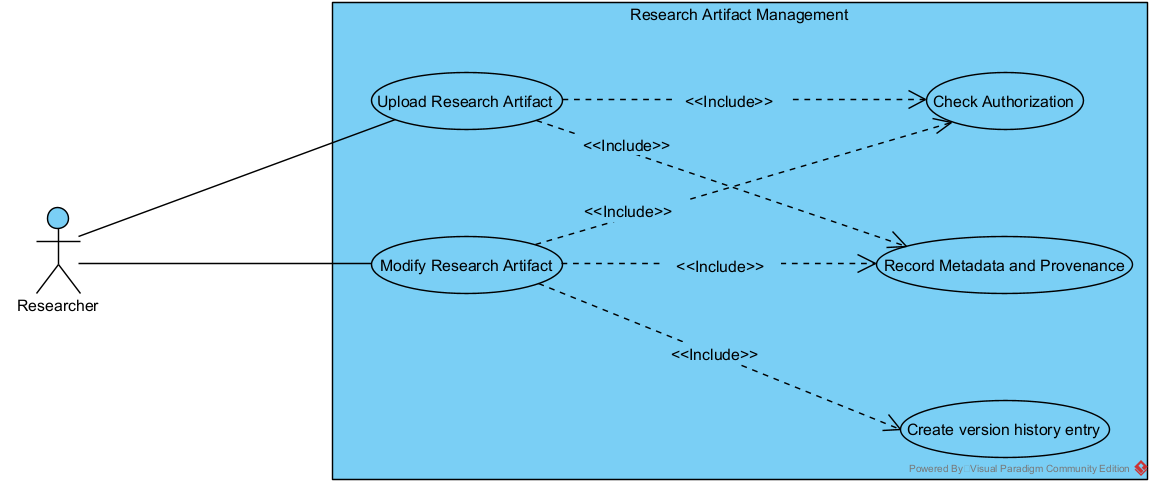
\includegraphics[width=1.05\textwidth,height=0.72\textheight,keepaspectratio]{png/UC-005 Use Case Diagram.png}
\caption{UC-005 Manage Research Artifacts Use Case Diagram}
\label{fig:uc005-usecase}
\end{figure}

\clearpage

\subsection{Activity Diagram}

The activity diagram shows the authorization decision,
artifact validation, success and failure paths,
and version-history creation.

\begin{figure}[htbp]
\centering
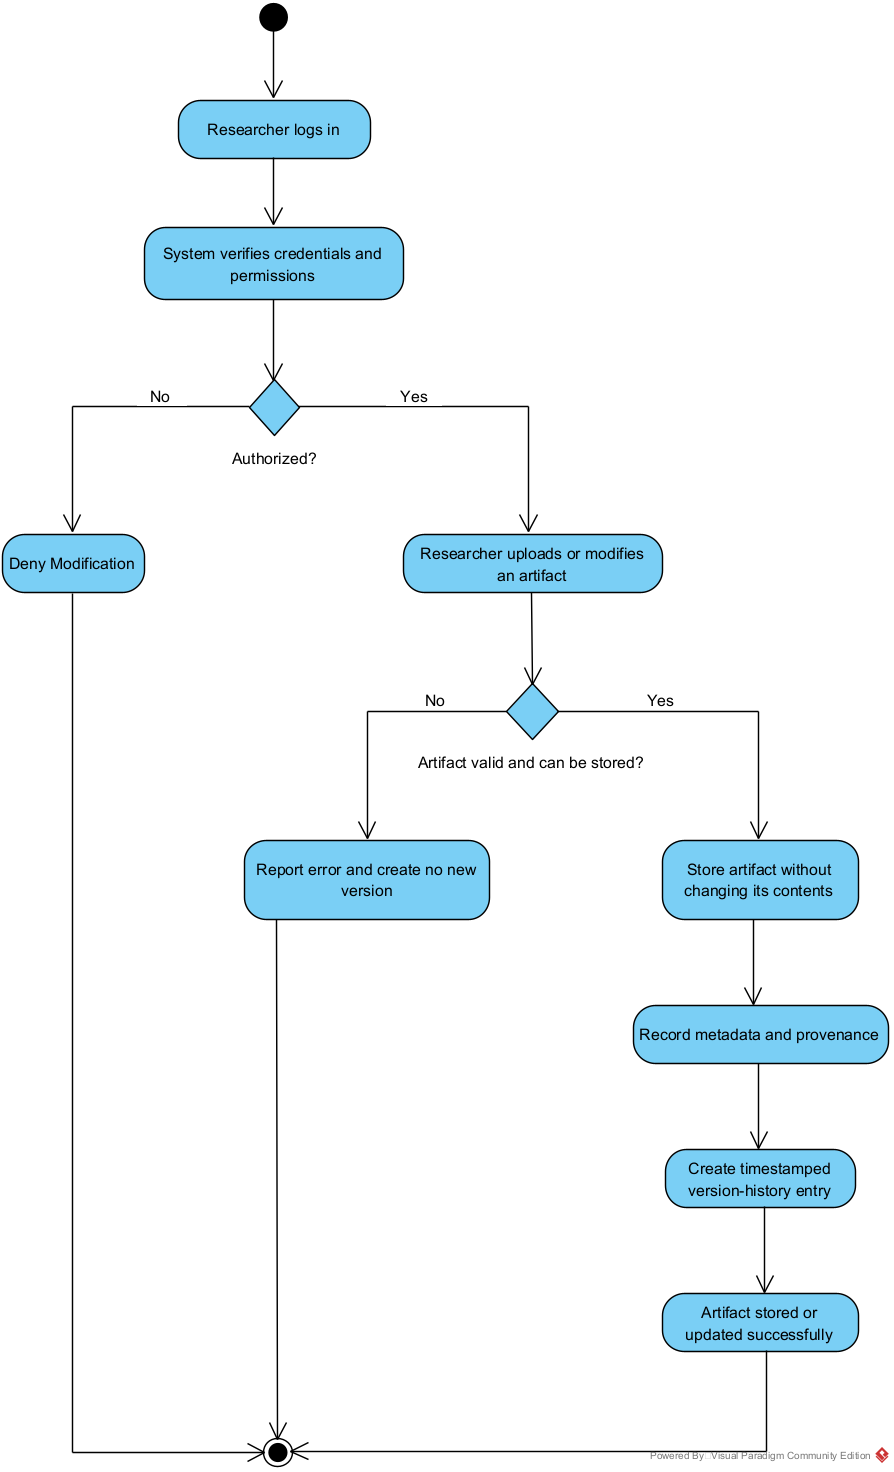
\includegraphics[width=0.8\textwidth,height=0.68\textheight,keepaspectratio]{png/UC-005ActivityDiagram.png}
\caption{UC-005 Manage Research Artifacts Activity Diagram}
\label{fig:uc005-activity}
\end{figure}

\clearpage

\subsection{Component Diagram}

The component diagram shows the React frontend,
Node.js and Express backend, authentication and
authorization, version management, ScyllaDB,
and file storage.

\begin{figure}[htbp]
\centering
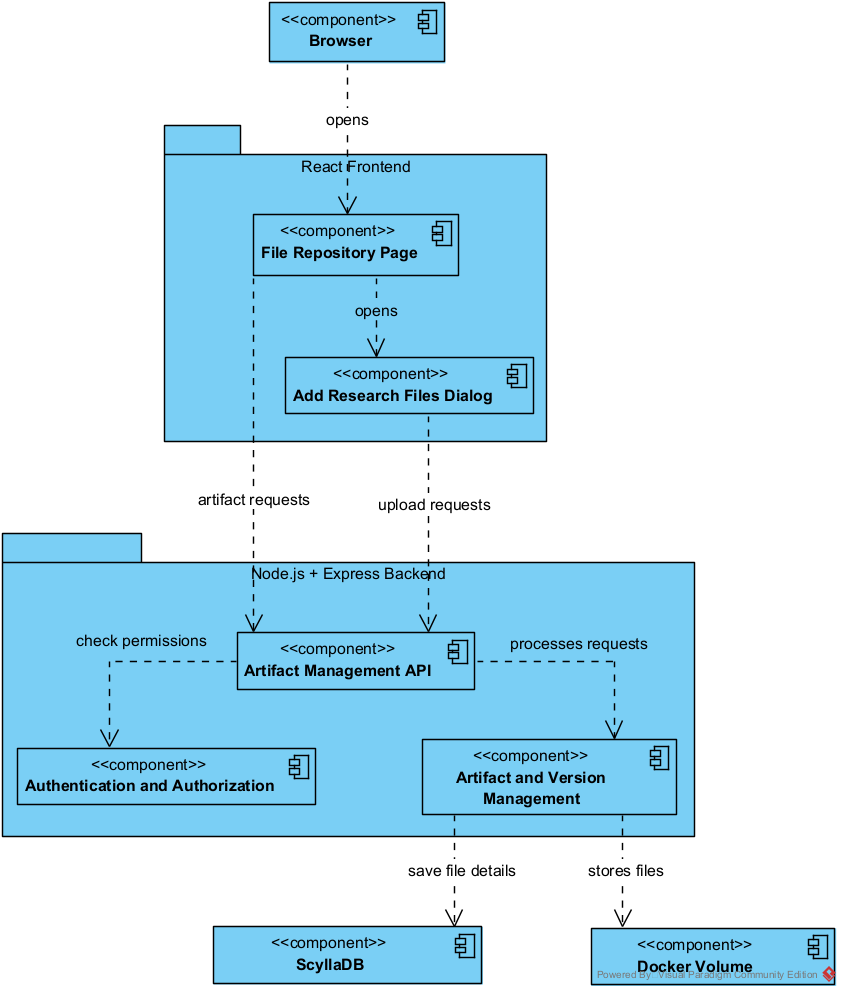
\includegraphics[width=0.95\textwidth,height=0.70\textheight,keepaspectratio]{png/UC-005 Component Diagram.png}
\caption{UC-005 Manage Research Artifacts Component Diagram}
\label{fig:uc005-component}
\end{figure}
\newpage
\subsection{MVC Diagram}

This diagram shows the interaction between the View, Controller, and Model of the platform
\begin{figure}[h!]
\centering
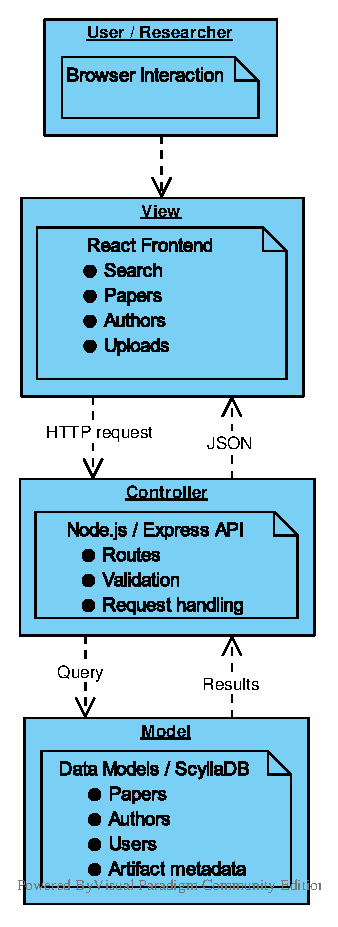
\includegraphics[width=0.35\textwidth]{eps/MVC_Diagram.eps}
\caption{MVC diagram of the Dynamo platform. \label{Figure:MVCDiagram}}
\end{figure}
\index{MVC Diagram}

\clearpage

%\chapter{Verification}
\ChapterLabel{Verification}
\index{verification}
\index{verification method}
\section{How to Use This Chapter}
Show that each requirement conforms to its specification using test, inspection, analysis, or demonstration. Record the method, evidence reference, responsible reviewer, result, and any waiver.
Verification answers ``Did we build the system right?''

\section{Verification Register}
\small
\begin{tabularx}{\linewidth}{L{1.8cm}L{2.6cm}L{2.0cm}YL{2.2cm}}
\caption{Verification Register\label{Table:VerificationRegister}}\\
\toprule
\textbf{ID} & \textbf{Requirement} & \textbf{Method} & \textbf{Required Evidence} & \textbf{Status}\\
\midrule
\endfirsthead
\multicolumn{5}{l}{\small\itshape Verification Register (continued)}\\
\toprule
\textbf{ID} & \textbf{Requirement} & \textbf{Method} & \textbf{Required Evidence} & \textbf{Status}\\
\midrule
\endhead
\midrule
\multicolumn{5}{r}{\small\itshape Continued on next page}\\
\endfoot
\bottomrule
\endlastfoot
\VerificationID{VER-001} & \RequirementRef{REQ-F-001} & Test & Passing \TestCaseRef{TC-001} execution record showing creation of one request with a unique identifier. & \StatusPass\\
\VerificationID{VER-002} & \RequirementRef{REQ-F-002} & Test & Passing \TestCaseRef{TC-002} execution record showing the current status and most recent update. & \StatusPass\\
\VerificationID{VER-003} & \RequirementRef{REQ-Q-001} & Analysis and test & Timing analysis and passing \TestCaseRef{TC-003} measurements under the reference workload. & \StatusPass\\
\VerificationID{VER-004} & \RequirementRef{REQ-F-003} & Inspection and test & Export inspection and passing \TestCaseRef{TC-004} execution record. & \StatusPending\\
\VerificationID{VER-005} & \RequirementRef{REQ-I-001} & Inspection and test & Schema-validation report and passing \TestCaseRef{TC-005} execution record. & \StatusPending\\
\VerificationID{VER-006} & \RequirementRef{REQ-S-001} & Analysis and test & Access-control analysis, denial records, and passing \TestCaseRef{TC-006} execution record. & \StatusPass\\
\VerificationID{VER-007} & \RequirementRef{REQ-D-001} & Inspection and test & Stored-history inspection and passing \TestCaseRef{TC-007} execution record. & \StatusPass\\
\VerificationID{VER-008} & \RequirementRef{REQ-C-001} & Test & Approved deployment baseline and passing \TestCaseRef{TC-008} compatibility results. & \StatusPass\\
\VerificationID{VER-009} & \RequirementRef{REQ-B-001} & Test & Timed analyst demonstration and passing \TestCaseRef{TC-009} execution record. & \StatusPending\\
\end{tabularx}
\normalsize

%\chapter{Validation}
\ChapterLabel{Validation}
\index{validation}
\index{validation scenario}
\section{How to Use This Chapter}
Evaluate whether the completed system solves stakeholder needs in its intended context. Define realistic scenarios, participant roles, success criteria, observations, and disposition of requested changes.
Validation answers ``Did we build the right system?''

\section{Validation Register}
\small
\begin{tabularx}{\linewidth}{L{1.6cm}L{2.4cm}YL{3.6cm}L{2.2cm}}
\caption{Validation Register\label{Table:ValidationRegister}}\\
\toprule
\textbf{ID} & \textbf{Related Story} & \textbf{Scenario} & \textbf{Success Criterion} & \textbf{Status}\\
\midrule
\endfirsthead
\multicolumn{5}{l}{\small\itshape Validation Register (continued)}\\
\toprule
\textbf{ID} & \textbf{Related Story} & \textbf{Scenario} & \textbf{Success Criterion} & \textbf{Status}\\
\midrule
\endhead
\midrule
\multicolumn{5}{r}{\small\itshape Continued on next page}\\
\endfoot
\bottomrule
\endlastfoot
\ValidationID{VAL-001} & \UserStoryRef{US-001} & A customer submits a realistic service request without coaching. & The customer receives a unique identifier and confirms that the workflow supports the intended task. & \StatusPending\\
\ValidationID{VAL-002} & \UserStoryRef{US-002} & A customer checks the progress of an existing request. & The customer correctly identifies the current status and latest update and judges the response timely. & \StatusPending\\
\ValidationID{VAL-003} & \UserStoryRef{US-003} & An authorized analyst exports a representative request history. & Within five minutes, the analyst opens the approved format, finds the expected records, and confirms source records were unchanged. & \StatusPending\\
\end{tabularx}
\normalsize


%\begin{dsnMilestone}[Milestone 3: Performance and Cost Review with Alpha Prototype Demonstration]
%Third week of February.
%\end{dsnMilestone}

%\chapter{Beta Prototyping: Design Revision and Optimization}\ChapterLabel{BetaPrototyping}
%\section{Mechanical Design}
%Describe mechanical revisions and optimizations made after alpha testing.
%\section{Electronics/Electro-Mechanical Design}
%Describe electrical and electro-mechanical revisions and optimizations made after alpha testing.
%\section{Software Design}
%Describe software revisions, defect corrections, performance improvements, and configuration changes.
%\section{System-Level Design}
%Describe integration changes, system-level optimization, and readiness for beta demonstration.

%\chapter{Fabrication, Assembly, and Manufacturing Processes}\ChapterLabel{FabricationAssemblyManufacturing}
%Document fabrication, assembly, manufacturing, quality-control steps, process outcomes, and lessons learned.

%\chapter{High-Performance Testing and Evaluation}\ChapterLabel{HighPerformanceTesting}
%Present final integrated-system tests under realistic user environments, results, limitations, and evidence that requirements are met.

%\begin{dsnMilestone}[Milestone 4: Optimized Design Review with Beta Prototype Demonstration]
%Last week of March: the design and prototype must be reasonably complete. The beta demonstration must integrate all subsystems into a fully functional system and demonstrate operation in realistic user environments.
%\end{dsnMilestone}

%\chapter{Final Design Specification}\ChapterLabel{FinalDesignSpecification}
%Provide the final controlled specification, final configuration, delivered design documents, requirements status, test evidence, known limitations, and acceptance status. Include detailed design documents in Appendix~D.

%\begin{dsnMilestone}[Milestone 5: Submission of the Final Report]
%Spring finals week.
%\end{dsnMilestone}
